\chapter{Centrales térmicas de carbón.}
\section{Esquema funcional de una central de carbón.}
Todas las centrales de combustible fósil clásicas tienen un esquema de funcionamiento prácticamente idéntico con las únicas diferencias siendo:
\begin{itemize}
	\item [-] El tratamiento previo del combustible.
	\item [-] El diseño de los quemadores.
	\item [-] El sistema de limpieza de humos y evacuación de las cenizas.
\end{itemize} 


Pese a ello, en la mayoría de centrales se pueden distinguir los siguientes circuitos básicos:
\begin{itemize}
	\item [-] Circuito de combustión.
	\item [-] Circuito aire-gases.
	\item [-] Circuito agua-vapor.
	\item [-] Circuito de agua de circulación.
	\item [-] Circuitos eléctricos.
	\item [-] Circuitos auxiliares.
\end{itemize}


\begin{figure}[H]
	\centering
	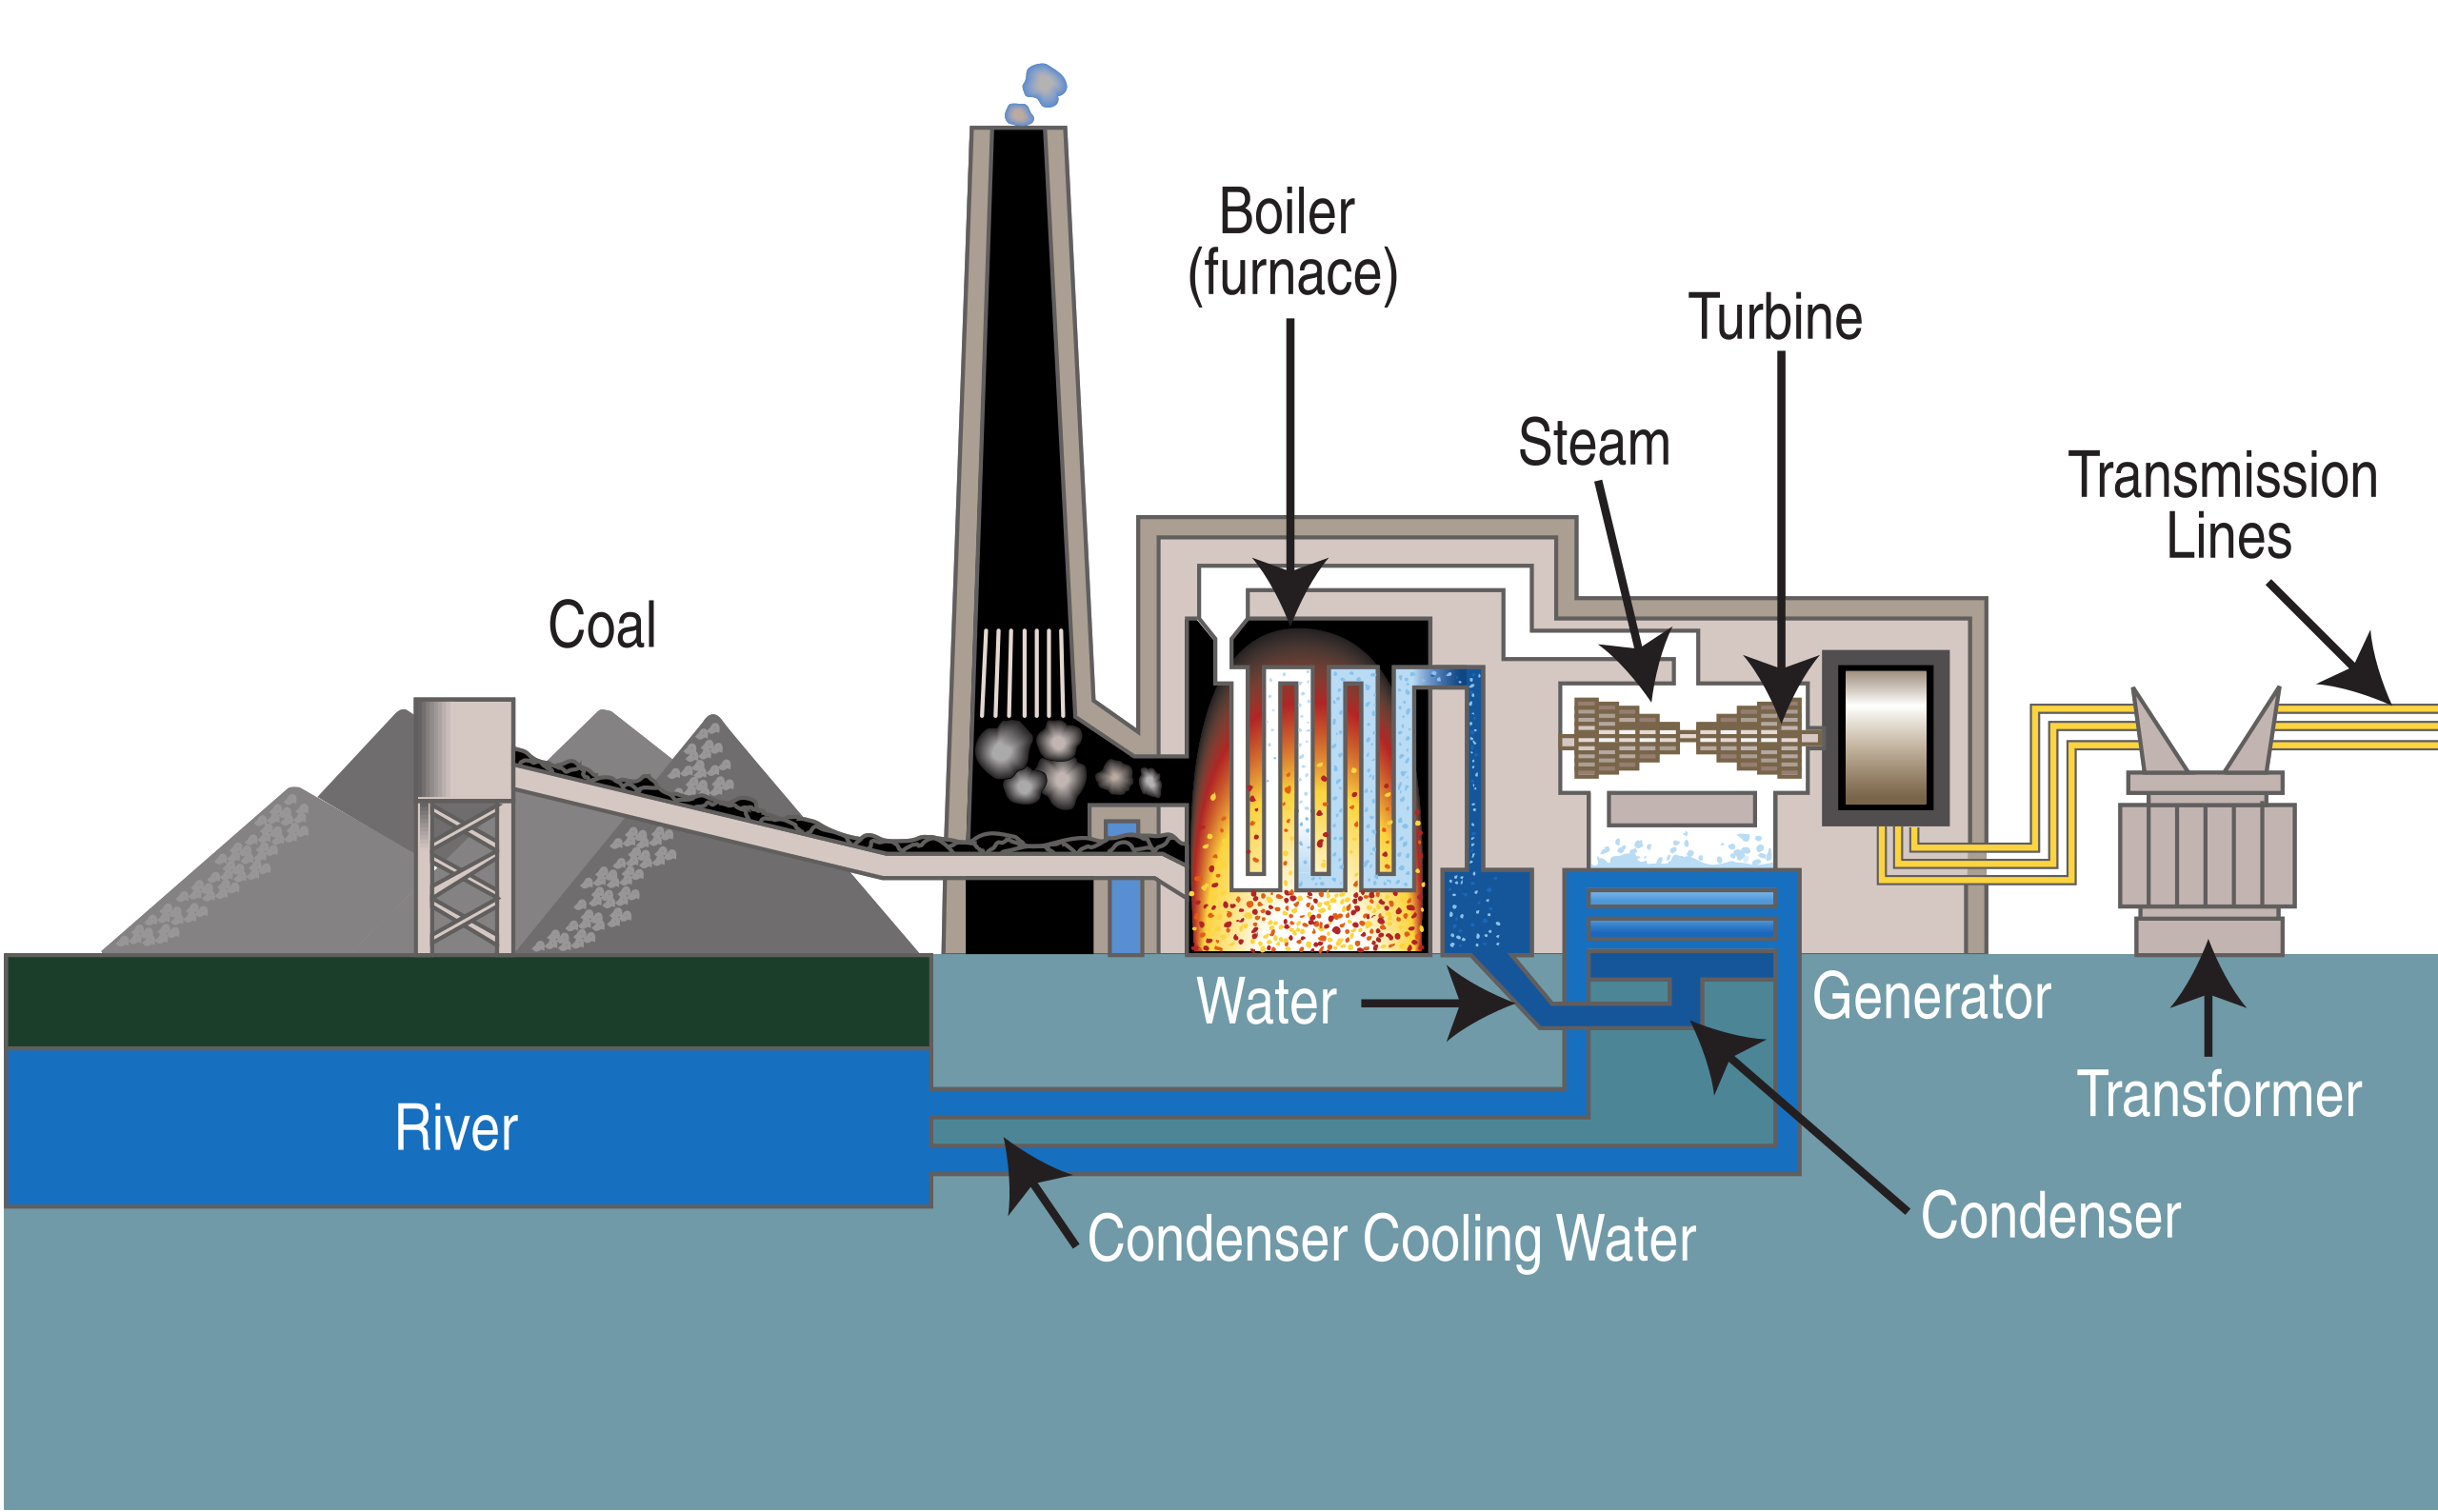
\includegraphics[width=0.7\linewidth]{res/tema10/esquemaFuncional}
	\label{fig:esquemafuncional}
\end{figure}

\section{Circuito aire-combustible-gases-ceniza.}
Este circuito se encarga de:
\begin{itemize}
	\item [-] Recibir y almacenar el combustible.
	\item [-] Preparar el combustible para ser quemado.
	\item [-] Transportar el combustible hasta el hogar.
	\item [-] Evacuación y filtrado de gases.
\end{itemize}
\section{Almacenamiento y preparación del combustible.}
\subsection{Almacenamiento del combustible.}
El almacenamiento se realiza en dos etapas. La primera etapa es el parque de combustible que suele tener una capacidad de almacenamiento de algunos meses de funcionamiento mientras que la segunda se compone por unos depósitos con capacidad para menos de un día.



El carbón se almacena en la cercanía de la central en parques a la intemperie y se maneja mediante rotopalas. Como se debe garantizar que haya un suministro esta la capacidad de almacenamiento suele ser elevada (hasta 150 días). Y si el carbón debe almacenarse más de un año se le proporciona un recubrimiento asfáltico.



No obstante, el almacenamiento de carbón presenta tres problemas principales:
\begin{itemize}
	\item [-] Combustión espontánea: debido al contacto con el aire el carbón se oxida a una velocidad proporcional a la temperatura (se duplica cada 8\grado). A los 65\grado $\ $ empieza a ser peligrosa y por tanto, el apilamiento debe hacerse de manera cuidadosa.
	\item [-] Pérdida de poder calorífica.
	\item [-] Degradación del tamaño del grano.
\end{itemize}


Del parque de almacenamiento se lleva el carbón a una torre de almacenamiento donde se separan las partículas férricas y trozos de piedras que pudiesen dañar los molinos. Tras pasar por la torre el carbón cae a través de las tolvas a unos alimentadores que dosifican la carga a los molinos.
\subsection{Preparación del combustible}
Una parte fundamental de la preparación del combustible consiste en pulverizar el carbón. 



Ventajas de la pulverización:
\begin{itemize}
	\item [-] Rendimiento de la combustión máximo.
	\item [-] Se pueden utilizar carbones de peor calidad.
	\item [-] Las cenizas y escorias no son pastosas (mejor manejo).
	\item [-] Mayor potencia calorífica por unidad de volumen del hogar. 
	\item [-] Menor costo de mano de obra.
 	\item [-] Fácil control del aire y combustible.
\end{itemize}





Desventajas de la pulverización:
\begin{itemize}
	\item [-] Elevado costo inicial de la instalación.
	\item [-] Costo de preparación del combustible.
	\item [-] Posibilidad de crear cenizas volantes (escapen por la chimenea).
\end{itemize}




Además, si el contenido de humedad es muy elevado el carbón antes de entrar al molino se mezcla con gas caliente para evaporar el agua.



Los molinos suelen transformar el carbón desde una granulometría menor a 150 mm hasta un grado de finura de aproximadamente 200$\mu m$ que depende del contenido en volátiles (a mayor contenido en volátiles mayor finura se requiere).



Una vez pulverizado la inyección puede ser:
\begin{itemize}
	\item [-] \textbf{Directa}: el carbón que sale de los molinos se lleva directamente a los quemadores. Es el método \textbf{más utilizado}.
	\item [-] \textbf{Indirecta}: el carbón se hace llegar a los molinos donde es transportado a unos silos de carbón pulverizado donde se almacena hasta que es inyectado en los quemadores.
\end{itemize}
\section{Tipos de molinos.}

\subsection{Molino de anillo de bolas.}
Es un tipo de molino donde un collar de esferas macizas de acero es arrastrado rondado entre dos anillos en los que hay talladas pistas troncotoroidales que guían a las bolas. La presión entre las bolas y anillos se mantiene mediante muelles de acero con una presión regulable.
\begin{figure}[H]
	\centering
	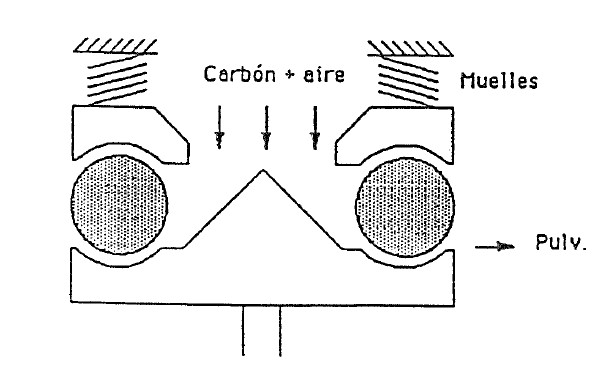
\includegraphics[width=0.4\linewidth]{res/tema10/molinoBolas}
	\label{fig:molinobolas}
\end{figure}

\subsection{Molino tubular de bolas tipo Hardinge.}
Es un molino que consta de un cilindro horizontal con bolas de acero en su interior que gira a velocidad constante. Se emplea aire caliente para secar el carbón y arrastrar el carbón pulverizado a un clasificador espiral.



Como las bolas se van desgastando con el tiempo ne van añadiendo en proporción 0,04-0,23 kg por tonelada de carbón pulverizado. Es un molino adecuado para antracitas aunque es ruidoso y es difícil controlar la finura del polvo. 



Estas calderas suelen absorber de 11 a 30$\frac{kWh}{ton}$ y pueden almacenar grandes cantidades de carbón para seguir suministrando carbón de 6 a 10 minutos.
\begin{figure}[H]
	\centering
	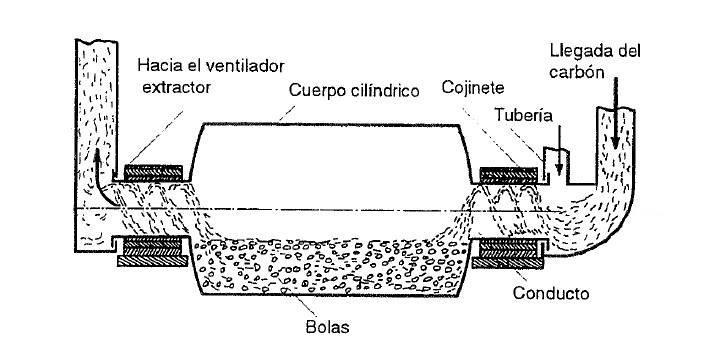
\includegraphics[width=0.6\linewidth]{res/tema10/molinoHardinge}
	\label{fig:molinohardinge}
\end{figure}

\subsection{Molino tubular de bolas Foster Wheeler.}
Es un molino muy simple, adecuado para antracitas. Es ruidoso y de velocidad limitada, pero permite controlar muy bien la finura de polvo. Puede almacenar gran cantidad de carbón.
\begin{figure}[H]
	\centering
	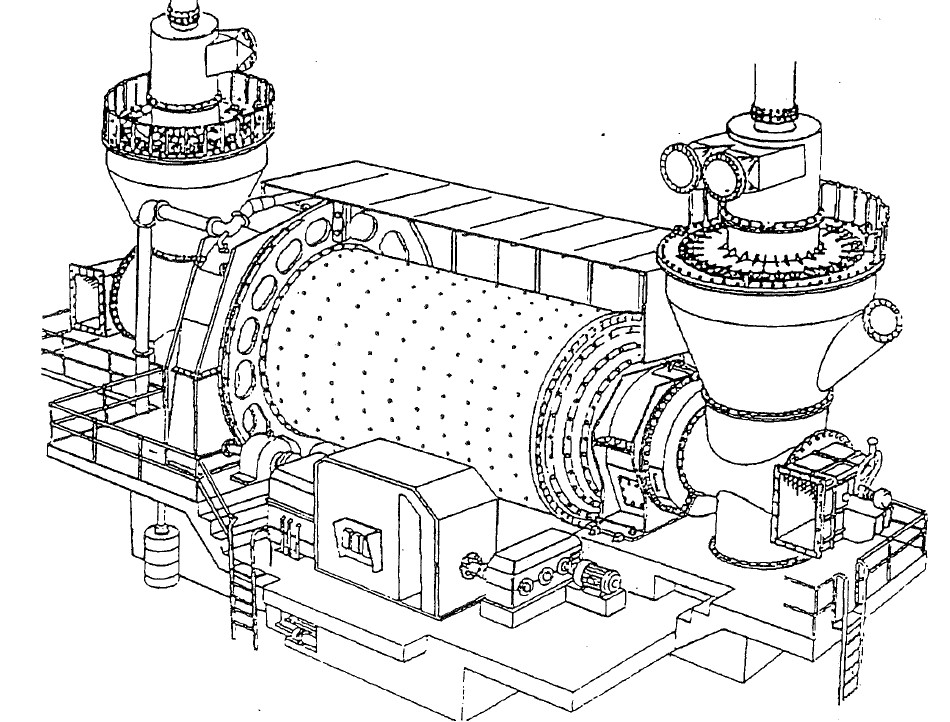
\includegraphics[width=0.4\linewidth]{res/tema10/fosterWheeler}
	\label{fig:fosterwheeler}
\end{figure}

\subsection{Molino de rodillos Babcock-Wilcox.}
Las bolas tienen un diámetro de 51 mm y su velocidad lineal es de 6$\frac{m}{s}$. El consumo de energía es de 8 a 12$\frac{kWh}{ton}$.
\begin{figure}[H]
	\centering
	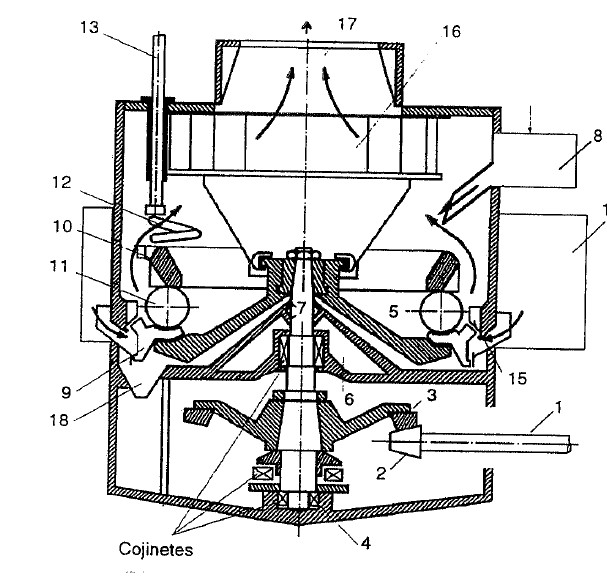
\includegraphics[width=0.3\linewidth]{res/tema10/babcock}
	\label{fig:babcock}
\end{figure}

\subsection{Molino de rodillos de Raymond.}
Este molino consta de tres rodillos que giran sobre un camino de rodadura. La presión correcta se consigue mediante unos muelles ajustables.


Tiene un bajo coste de mantenimiento y es silencioso. Puede triturar 70$\frac{t}{h}$ de carbón pulverizado. Absorbe entre 11 y 16$\frac{kWh}{ton}$.
\begin{figure}[H]
	\centering
	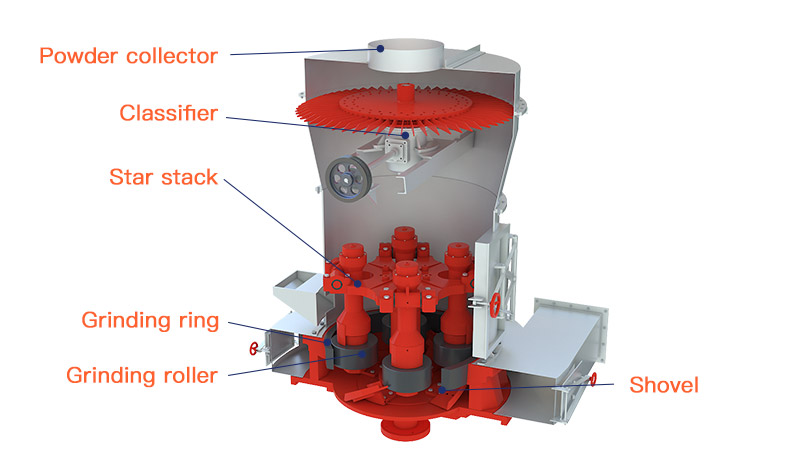
\includegraphics[width=0.5 \linewidth]{res/tema10/raymond}
	\label{fig:raymond}
\end{figure}

\subsection{Molino de batea móvil.}
Es un molino  con una batea móvil con forma troncocónica que gira alrededor de un eje vertical a una velocidad entre 65 y 100 rpm. En su interior se alojan tres muelas cónicas tangentes a la superficie de la batea que giran solidariamente entre sí.




El carbón entra por el centro en el espacio que dejan libres las muelas que a través de la fuerza centrífuga es lanzado contra las paredes donde es triturado por las muelas.


Para extraer este carbón, se emplea aire precalentado que arrastra el carbón pulverizado hacia un separador y las partículas gruesas vuelven al molino.


Este molino tiene bajo costo de mantenimiento y bajo consumo de energía.

\begin{figure}[H]
	\centering
	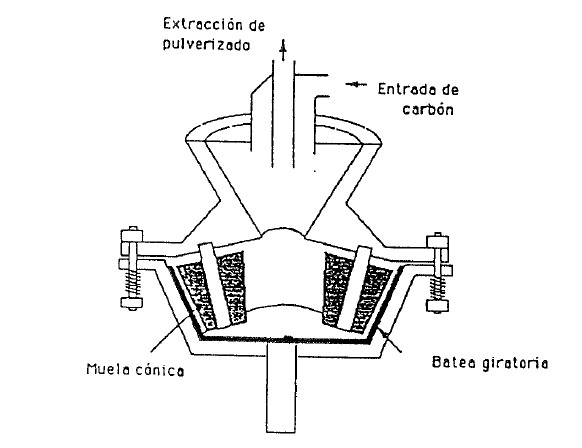
\includegraphics[width=0.5\linewidth]{res/tema10/bateaMovil}
	\label{fig:bateamovil}
\end{figure}


\subsection{Molinos de tipo impacto.}
Este tipo de molinos emplea anillos cilíndricos que giran a una velocidad entre 1000 y 2000 rpm. Dos de los anillos son trituradores y otros dos son lisos para arrastrar el carbón.


A diferencia de anteriores molinos, el carbón descarga directamente por la parte inferior a través de una parrilla que asegura la granulometría deseada.
\begin{figure}[H]
	\centering
	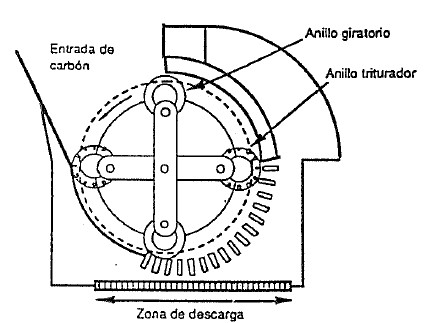
\includegraphics[width=0.5\linewidth]{res/tema10/impacto}
	\label{fig:impacto}
\end{figure}

\section{Circuito aire-gases.}
El aire tomado de la atmósfera se envía mediante ventiladores de tiro forzado a través de precalentadores.

El objetivo de los quemadores:
\begin{itemize}
	\item [-] Recuperar el calor contenido en los gases a la salida de los intercambiadores de agua y vapor.
	\item [-] Elevar la temperatura del aire empleado en la combustión para mejorarla y, para secar el carbón.
\end{itemize}


A la salida de los precalentadores, el aire se envía a la cámara de combustión de diferentes manera:
\begin{itemize}
	\item [-] A través de los quemadores como aire primario mezclado con el combustible.
	\item [-] Alrededor de los quemadores como aire secundario.
	\item [-] A lo largo del recorrido de la llama como aire terciario.
\end{itemize}

\begin{figure}[H]
	\centering
	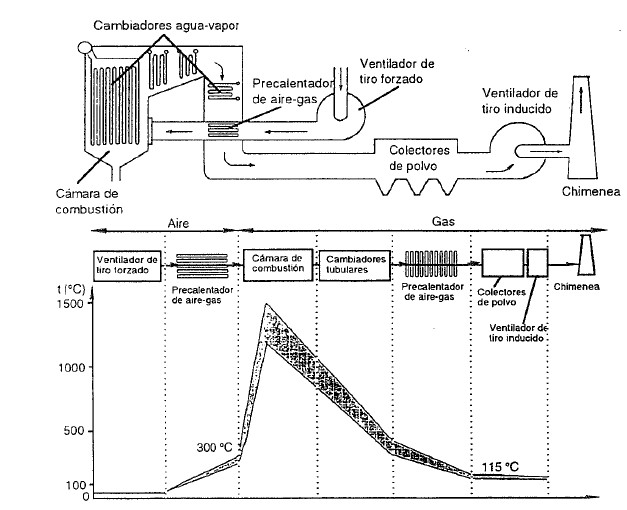
\includegraphics[width=0.7\linewidth]{res/tema10/circuitoAwaGas}
	\label{fig:circuitoawagas}
\end{figure}

\section{Quemadores.}
Los mecheros o quemadores son dispositivos mediante los cuales se introduce carbón pulverizado en suspensión en el aire primario hacia el hogar. Estos dispositivos deben permitir:
\begin{itemize}
	\item [-] El ajuste del punto de ignición.
	\item [-] La estabilidad de la llama (la velocidad de la mezcla aire-carbón iguala a la de propagación de la llama).
	\item [-] La combustión completa.
 	\item [-] La distribución uniforme del exceso de aire y de la temperatura.
	\item [-] El fácil acceso para el mantenimiento.
\end{itemize}



Los quemadores constan de varios conductores donde uno es para el fuel (precalentar el hogar), otro es para el carbón y aire primario y uno adicional para el aire secundario. Además, los quemadores son orientables y se puede modificar su ángulo de incidencia para el control de la combustión.
\begin{figure}[H]
	\centering
	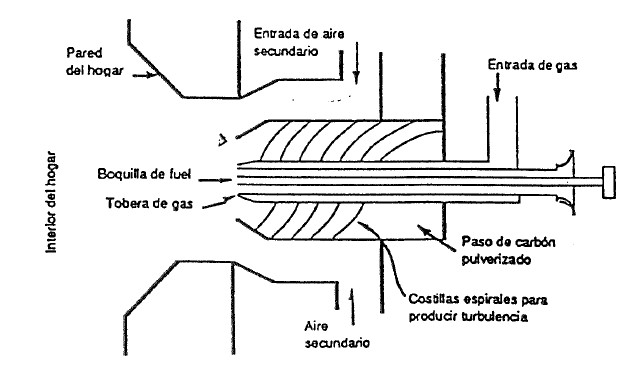
\includegraphics[width=0.6\linewidth]{res/tema10/boquilla}
	\label{fig:boquilla}
\end{figure}


En función del tipo de flujo se tienen:
\begin{itemize}
	\item [-] \textbf{Quemadores de tipo laminar}: las turbulencias se producen por la propia velocidad de la muestra, por el uso de deflectores y por la entrada de aire secundario y terciario.
	\item [-] \textbf{Quemadores de turbulencias}: se imprime un movimiento rotativo al flujo de carbón y aire primario.
\end{itemize}


Para precalentar el hogar de la caldera se emplea combustible líquido (fuel-oil).
\section{Hogar.}
Es la parte de la caldera donde tiene lugar la combustión. El calor desprendido se transmite primero por radiación a todas las partes que están en presencia de la llama y, posteriormente a las partes de la caldera que no ven el fuego mediante convección denominada zona de recuperación de calor (camino de salida de los humos).
\subsection{Pantallas evaporadoras.}
El hogar de una caldera es un volumen diáfano de grandes dimensiones cuyas paredes están
constituidas habitualmente por paneles verticales de tubos soldados de aletas longitudinales
(pantallas evaporadoras). Normalmente van dispuestos verticalmente, soldados a los colectores
extremos (entrada inferior y salida superior).




Por el interior de estos paneles asciende agua de alimentación precalentada a 100\grado $\ $ procedente del economizador, a través de tubos recubiertos de materiales refractarios que bajan desde la parte superior de la caldera (downcommers) que actúa como fluido refrigerante de los propios tubos.


Las paredes de agua van fijas a la envolvente de la caldera de modo que permita su libre
dilatación. 


La envolvente de la caldera es chapa metálica mientras el aislamiento térmico de las paredes
es cemento refractario o roca de vidrio
\section{Ventiladores.}
Para regular la presión en el interior del hogar se emplean ventiladores de tiro forzado que impulsan el aire al interior del hogar para proporcionar presión suficiente para vencer las pérdidas de carga en el circuito aire-gas. No obstante, si la presión en el interior del hogar es menor a la atmosférica (depresión) es necesario un segundo ventilador, de tiro inducido, para aspirar los gases de la combustión y enviarlos a la chimenea.



Las calderas de combustible sólido suelen estar en depresión y las de combustibles líquidos o gaseosos son presurizados.



la geometría de los ventiladores, suele ser de tipo centrífugo donde el aire entra paralelamente al eje y sale de forma radial por medio de una cámara espiral. En estos ventiladores se cumple:
\[Gasto \ másico \propto velocidad\]
\[Presión\propto velocidad^2\]
\[Potencia\propto velocidad^3\]


\subsection{Ventiladores de tiro forzado.}
Se introduce aire a presión al hogar de forma que se vencen los rozamientos y las pérdidas de carga en todo el recorrido de los gases de combustión.
\begin{figure}[H]
	\centering
	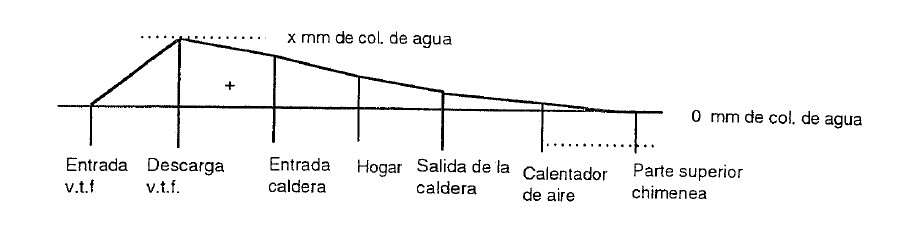
\includegraphics[width=0.7\linewidth]{res/tema10/forzao}
	\label{fig:forzao}
\end{figure}

\subsection{Ventiladores de tiro inducido.}
Se colocan dos por seguridad y se encargan de aspirar los gases del hogar y los envían a la chimenea.
\begin{figure}[H]
	\centering
	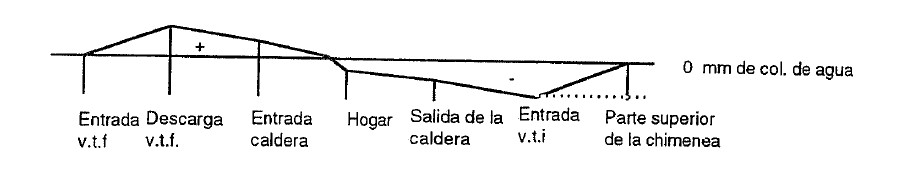
\includegraphics[width=0.7\linewidth]{res/tema10/inducio}
	\label{fig:inducio}
\end{figure}

\section{Precalentadores.}
Su misión es recuperar parte del calor de los gases de combustión para volver a introducirlos en la caldera. De esta forma se aumenta el rendimiento entre un 2,3 y un 2,6\% y un ahorro de combustible entre el 5 y 10\%.



Los precalentadores pueden de tipo:
\begin{itemize}
	\item [-] \textbf{Recuperativo}: los gases y el aire están separados por una pared metálica que transmite el calor.
	\item [-] \textbf{Regenerativo}: la superficie metálica es calentada y enfriada por los gases y el aire de manera alternada. Si tienen un tambor fijo y giran los tubos se denominan de Rothemüle y si el proceso es inverso se denominan de Ljungstrom. 
\end{itemize}
\begin{figure}[H]
	\centering
	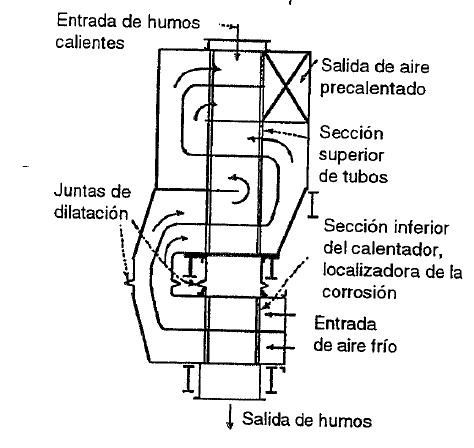
\includegraphics[width=0.4\linewidth]{res/tema10/precalentador}
	\label{fig:precalentador}
\end{figure}



\section{Productos de desecho: Cenizas volantes y escoria.}
El tratamientos para otros productos de desecho de las centrales (gases principalmente) se discutieron en los capítulos 2 y 3. 


Cuando se habla de cenizas volantes y escorias se refiere a compuestos inorgánicos que no se descomponen a la temperatura del hogar pero si se funden. Se diferencia entre las cenizas volantes y la escoria reside en el grosor de estas aglomeraciones. La proporción cenizas volantes y escorias es 4:1 respectivamente.





 Aunque la composición de materia inorgánica varia enormemente según la clase de carbón se pueden establecer los siguientes valores orientativos:
\begin{table}[H]
	\centering
	\renewcommand{\arraystretch}{1.5}
	\begin{tabular}{|c|c|}
		\hline
		Compuesto&$\%$  en peso\\
		\hline
		$SiO_2$&$50,8-32,9$\\
		\hline
		$Al_2O_3$&$30,6-15,1$\\
		\hline
		$Fe_2O_3$&$11,0-32,9$\\
		\hline
		$CaO$&$5,0-8,4$\\
		\hline
		$Na_2O+K_2O$&$2,0-3,0$\\
		\hline
		$MgO$&$0,6-0,8$\\
		\hline
	\end{tabular}
\end{table}



\subsection{Ceniceros.}
Son recipientes diseñados para enfriar las cenizas y evacuarlas al exterior.




En función del tipo de funcionamiento se diferencian entre húmedo y seco. A su vez, los de tipo húmedo se diferencian entre los de funcionamiento continuo (tipo alemán) y funcionamiento intermitente (tipo americano).
\begin{figure}[H]
	\begin{minipage}{0.55\textwidth}
		\centering
		\textbf{Cenicero de tipo alemán.}
		\begin{figure}[H]
			\centering
			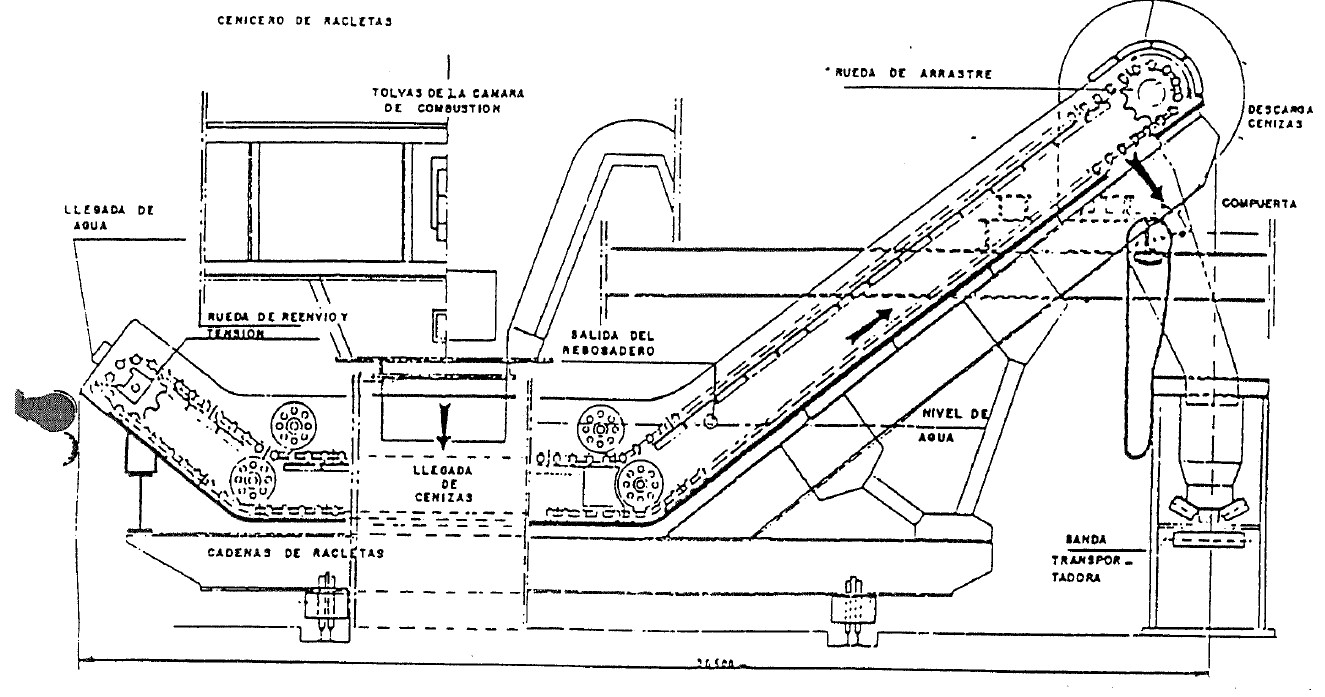
\includegraphics[width=1\linewidth]{res/tema10/aleman}
			\label{fig:aleman}
		\end{figure}
	\end{minipage}
	\begin{minipage}{0.45\textwidth}
		\centering
		\textbf{Cenicero de tipo americano.}
		\begin{figure}[H]
			\centering
			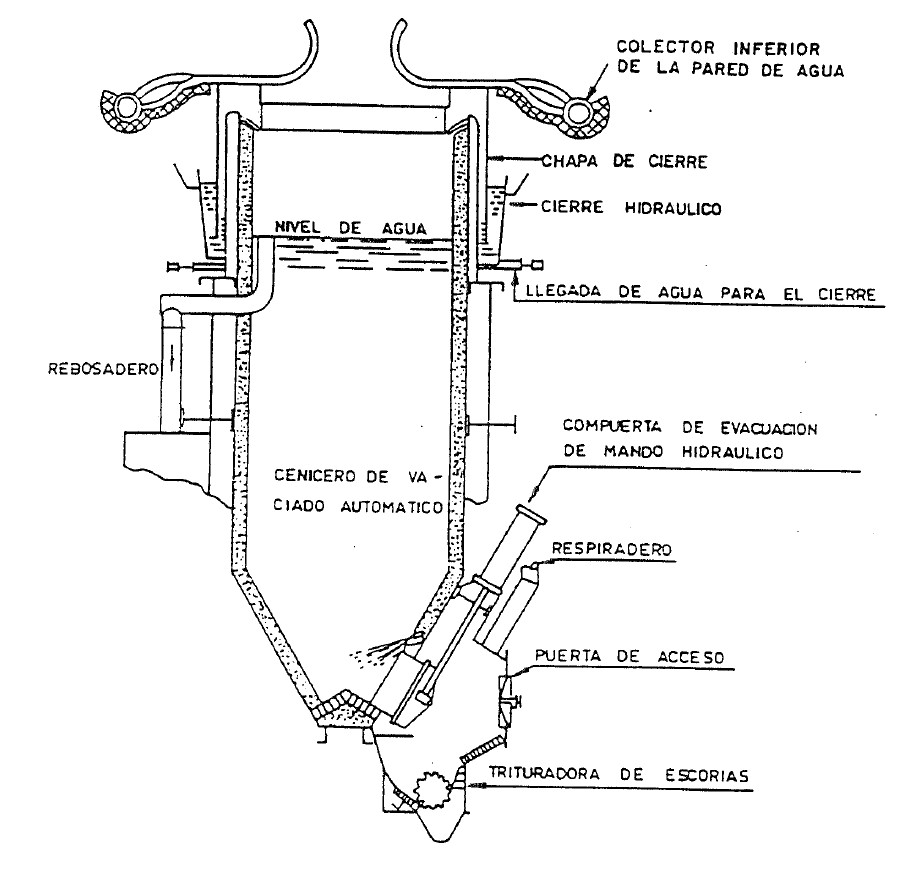
\includegraphics[width=0.7\linewidth]{res/tema10/americano}
			\label{fig:americano}
		\end{figure}
	\end{minipage}
\end{figure}	





\subsection{Retención de cenizas volantes.}
La extracción de de las cenizas volantes se efectúa mediante tolvas colectoras situadas en distintos puntos del circuito aire-gas:
\begin{table}[H]
	\centering
	\renewcommand{\arraystretch}{1.5}
	\begin{tabular}{|c|c|}
		\hline
		Punto&$\%$ de ceniza recogida\\
		\hline
		Precipitador electrostático&$60$\\
		\hline
		Precipitador mecánico&$25$\\
		\hline
		Precalentador de aire&$7$\\
		\hline
		Economizador&$5$\\
		\hline
		Base de la chimenea&$3$\\
		\hline
	\end{tabular}
\end{table}


El principal problema que existe con el contenido en polvo de los gases de combustión es su extremada finura ($50\mu m$). Por ello, para limitar la evacuación de polvo a la atmósfera se emplean filtros mecánicos, electrostáticos o mixtos.
\subsubsection{Filtros mecánicos.}
Separan las partículas más pesadas por cambios de dirección (filtros en zigzag) o por fuerza centrífuga (filtros ciclón). Las partículas intermedias son retenidas por filtros de mangas y las más finas por los electrostáticos.
\begin{figure}[H]
	\begin{minipage}{0.55\textwidth}
El filtrado se puede producir en la masa del material y cuando se colmata hay que sustituirle o bien en su superficie, permitiendo su limpieza. Para ello, se elige recubrir con una capa de Gore-Tex (teflón microporoso).	
\end{minipage}
\begin{minipage}{0.45\textwidth}
\begin{figure}[H]
	\centering
	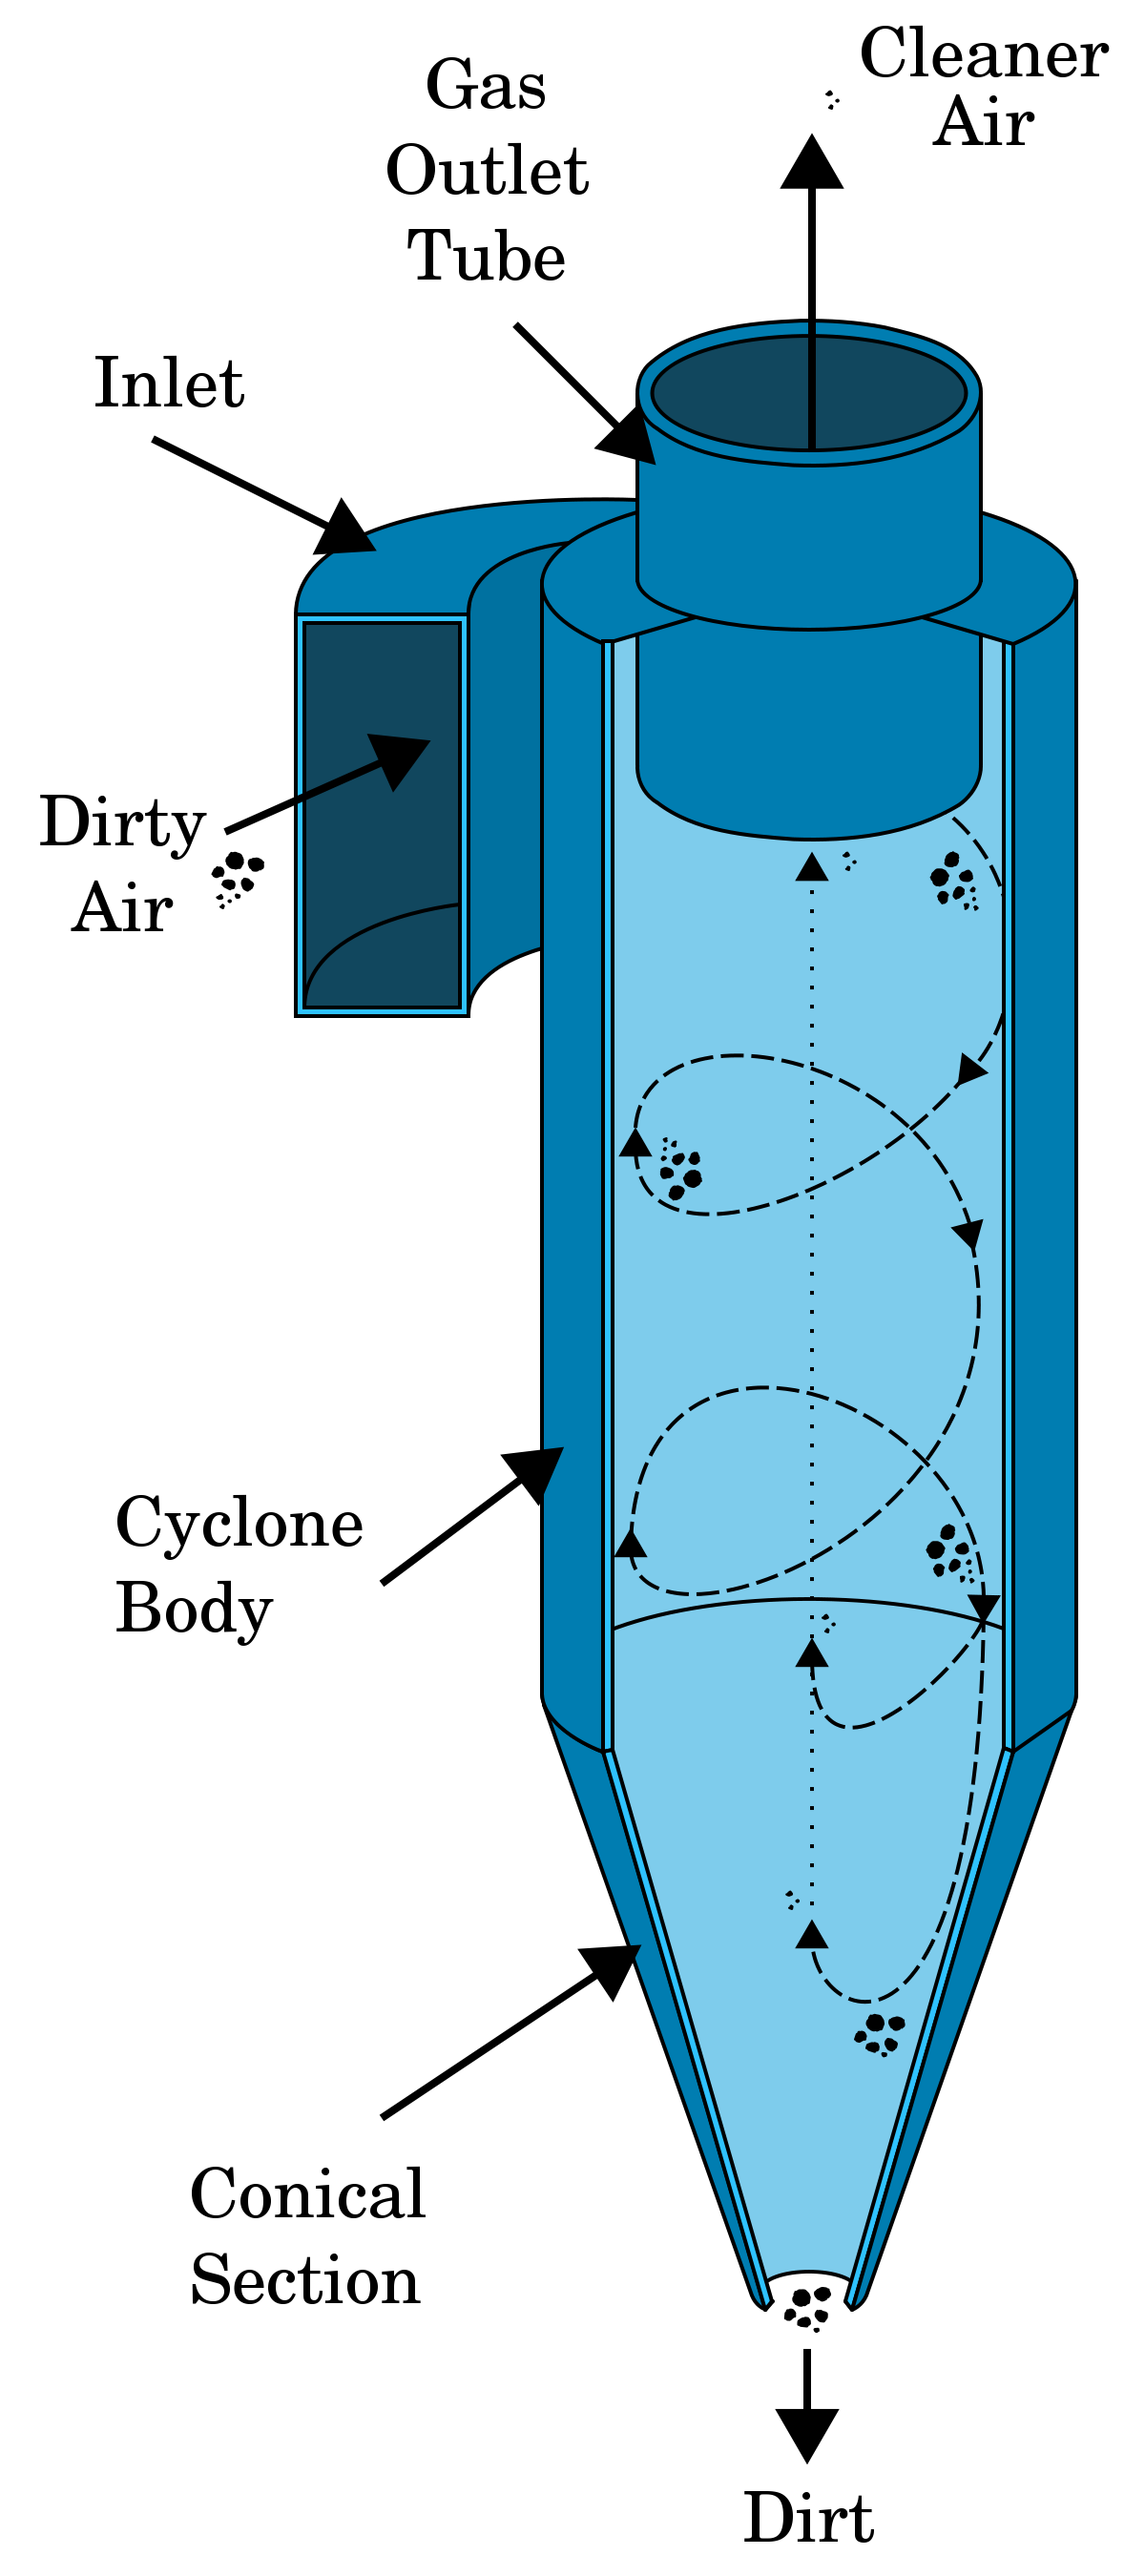
\includegraphics[width=0.4\linewidth]{res/tema10/ciclo9n}

	\label{fig:ciclo9n}
\end{figure}
	\end{minipage}
\end{figure}



\subsubsection{Filtros electrostáticos.}
Se basan en ionizar las partículas mediante un campo eléctrico elevado que posteriormente serán atraídas por los electrodos. Suelen a funcionar entre tensiones de 20 y 100kV y consumir entre 600 y 800kW para una planta de 400MW.
\begin{figure}[H]
	\centering
	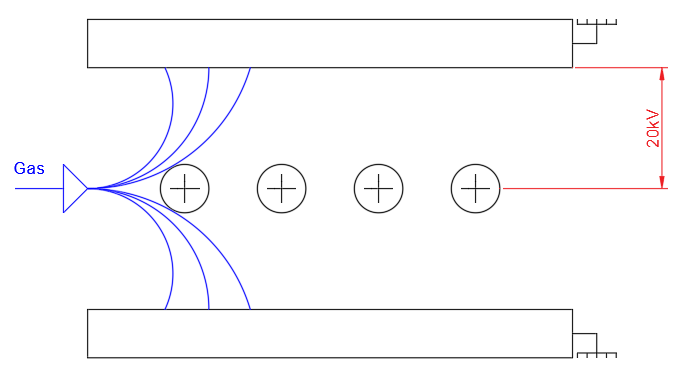
\includegraphics[width=0.7\linewidth]{res/tema2/filtroelectrostatico}
	\label{fig:filtroelectrostatico}
\end{figure} 
\subsubsection{Colectores mixtos.}
Son filtros electromecánicos y utilizan una separación escalonada. A la entrada se coloca el colector mecánico para atrapar las partículas mecánicas y a continuación el electrostático.
\begin{figure}[H]
	\centering
	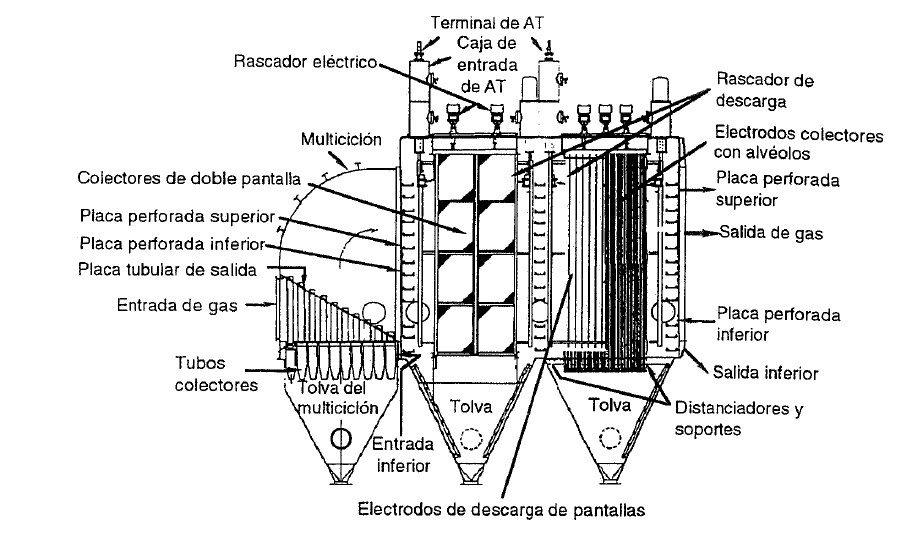
\includegraphics[width=0.7\linewidth]{res/tema10/colectorMixto}
	\label{fig:colectormixto}
\end{figure}

\section{Chimenea.}
Los gases de escape de la combustión, una vez enfriados en los precalentadores hasta cerca de 130 °C
y filtrados en los precipitadores, son aspirados por los ventiladores de tiro inducido y descargados a la
atmósfera por las chimeneas.


La construcción de las chimeneas es de doble pared: la interior con tramos de idéntica sección y
altura, construida con material refractario, y el fuste exterior de hormigón de sección decreciente y
construido en una sola pieza por fraguado continuo.



Las chimeneas son diseñadas para asegurar, en todo momento, que los gases emitidos no van a
afectar la calidad del aire ambiente, a nivel del suelo.

\section{Circuito agua vapor.}
El circuito agua vapor esta compuesto por todos los elementos que participan en el ciclo termodinámico realizado mediante el uso de agua. Este ciclo funciona en circuito cerrado salvo pequeñas pérdidas y desde el punto de vista técnico se suele trabajar a presiones de 180 bar y temperaturas de 550\grado.




Los elementos que forman el circuito son:
\begin{itemize}
	\item [-] Pantallas evaporadoras.
 	\item [-] Sobrecalentador.
 	\begin{itemize}
 		\item Sobrecalentador primario de radiación.
 		\item Sobrecalentador secundario de convección.
 	\end{itemize}
	\item [-] Recalentadores.
	\begin{itemize}
		\item Recalentador primario.
		\item Recalentador secundario.
		\item Recalentador terciario.
	\end{itemize}
	\item [-] Economizador.
	\item [-] Calderín.
	\item [-] Turbina de vapor.
	\begin{itemize}
		\item Cuerpo de alta presión.
		\item Cuerpo de media presión.
		\item Cuerpo de baja presión.
	\end{itemize}
	\item [-] Condensador.
	\item [-] Desgasificador.
	\item [-] Precalentadores de agua de alimentación de la caldera.
	\item [-] Bomba de alimentación agua caldera.
\end{itemize}





\begin{figure}[H]
	\centering
	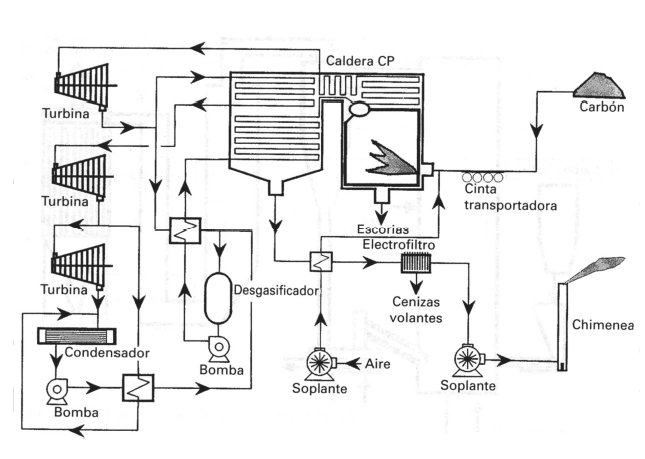
\includegraphics[width=0.7\linewidth]{res/tema10/awaVapor}
	\label{fig:colectormixto}
\end{figure}

\section{Ciclo de Rankine.}
Es el ciclo principal empleado para obtener energía útil a partir del carbón. En las figuras siguientes se puede ver el ciclo básico tanto en diagrama TS como en su ejecución.


\begin{figure}[H]

		
	\begin{minipage}{0.5\textwidth}
		 \begin{adjustbox}{width=1\textwidth}
			\centering
			\begin{circuitikz}
				\tikzstyle{every node}=[font=\normalsize]
				\draw  (3,11.5) circle (0.25cm);
				\draw [short] (2.75,11.5) -- (2.5,11);
				\draw [short] (2.5,11) -- (3.5,11);
				\draw [short] (3.5,11) -- (3.25,11.5);
				\draw [short] (3.25,11.5) -- (5.25,11.5);
				\draw [short] (3,11.75) -- (3,13.25);
				\draw  (5.25,11.75) rectangle (7.25,10.75);
				\draw [short] (7.25,11) -- (9.25,11);
				\draw [short] (9.25,11) -- (9.25,12.75);
				\draw [short] (8.5,13) -- (9.25,12.75);
				\draw [short] (9.25,12.75) -- (10,12.5);
				\draw [short] (10,12.5) -- (10,13.75);
				\draw [short] (8.5,13) -- (8.5,13.5);
				\draw [short] (10,13.75) -- (10,14);
				\draw [short] (8.5,13.5) -- (10,14);
				\draw [short] (9.25,13.75) -- (9.25,15);
				\draw [short] (9.25,15) -- (7.5,15);
				\draw [short] (7.25,15.5) .. controls (7.5,15.25) and (7.5,14.5) .. (7.25,14.5);
				\draw [short] (5.25,14.5) .. controls (5,14.5) and (5,15.25) .. (5.25,15.5);
				\draw [short] (5.25,14.5) -- (7.25,14.5);
				\draw [short] (7.25,15.5) -- (5.25,15.5);
				\draw [short] (5,15) -- (3,15);
				\draw [short] (3,15) -- (3,13);
				\draw [short] (10,13.5) -- (10.75,13.5);
				\draw [short] (10,13) -- (10.75,13);
				\draw  (11.25,13.25) circle (0.5cm) node {\normalsize G} ;
				\draw [->, >=Stealth, dashed] (1.75,11.5) -- (2.75,11.5);
				\draw [->, >=Stealth, dashed] (6.25,10.75) -- (6.25,9.75);
				\draw [->, >=Stealth, dashed] (6.25,16.5) -- (6.25,15.5);
				\draw [->, >=Stealth, dashed] (10.25,14) -- (11.5,14);
				\node [font=\normalsize] at (6.25,16.75) {$Q_C$};
				\node [font=\normalsize] at (6.25,9.5) {$Q_F$};
				\node [font=\normalsize] at (10.5,14.5) {$W_{TV}$};
				\node [font=\normalsize] at (1.75,11.75) {$W_B$};
				\node [font=\normalsize] at (9.25,13.25) {TV};
				\node [font=\normalsize] at (3,11.5) {B};
				\node [font=\normalsize] at (6.25,11.25) {Cond};
				\node [font=\normalsize] at (6.25,15) {Cald};
				\draw [short] (4.25,11.75) -- (4.25,11.25);
				\draw [short] (4.25,14.75) -- (4.25,15.25);
				\draw [short] (8.25,11.25) -- (8.25,10.75);
				\draw [short] (8.25,14.75) -- (8.25,15.25);
				\node [font=\normalsize] at (8.25,15.5) {1};
				\node [font=\normalsize] at (8.25,11.5) {2};
				\node [font=\normalsize] at (4.25,12) {3};
				\node [font=\normalsize] at (4.25,15.5) {4};
			\end{circuitikz}
			\label{fig:my_label}
			 \end{adjustbox}
	\end{minipage}
	\begin{minipage}{0.5\textwidth}
	 \begin{adjustbox}{width=0.8\textwidth}
		\centering	
		\begin{circuitikz}
			\tikzstyle{every node}=[font=\normalsize]
			\draw [->, >=Stealth] (3.5,10) -- (3.5,16.25);
			\draw [->, >=Stealth] (3,10.5) -- (11,10.5);
			\node [font=\normalsize] at (11.25,10.5) {S};
			\node [font=\normalsize] at (3.5,16.5) {T};
			\draw [short] (4.25,11) .. controls (5.25,13) and (5.75,15) .. (6.75,15);
			\draw [short] (6.75,15) .. controls (7.75,14.75) and (8.25,13) .. (10,11.5);
			\draw [->, >=Stealth, dashed] (5.25,13.25) -- (8.5,13.25);
			\draw [->, >=Stealth, dashed] (8.5,13.25) -- (8.5,11.5);
			\draw [->, >=Stealth, dashed] (8.5,11.5) -- (4.5,11.5);
			\draw [->, >=Stealth, dashed] (4.5,11.5) -- (4.5,12.25);
			\draw [->, >=Stealth, dashed] (4.5,12.25) -- (5.25,13.25);
			\node [font=\normalsize] at (8.75,13.5) {1};
			\node [font=\normalsize] at (8.5,11.25) {2};
			\node [font=\normalsize] at (4.5,11) {3};
			\node [font=\normalsize] at (4.25,12.25) {4};
		\end{circuitikz}
		\label{fig:my_label}
	 \end{adjustbox}
	\end{minipage}
\end{figure}
Las distintas etapas del ciclo son:
\begin{itemize}
	\item [-] Proceso 1$\rightarrow$2. Expansión isoentrópica del vapor en la turbina. $\dot{W}_{TV}=h_1-h_2$.
	\item [-] Proceso 2$\rightarrow$3. Condensación isobárica del vapor en el condensador. $\dot{q}_F=h_2-h_3$.
	\item [-] Proceso 3$\rightarrow$4. Compresión isoentrópica en la bomba. $\dot{W}_B=h_4-h_3=\frac{P_4-P_3}{\rho}$.
	\item [-] Proceso 4$\rightarrow$1. Calentamiento isobárico en la caldera. $\dot{q}_C=h_1-h_4$.
\end{itemize}

El rendimiento por otro lado:
\[\eta=\frac{\dot{W}_{TV}-|\dot{W}_B|}{\dot{q}_C}=1-\frac{\dot{q}_F}{\dot{q}_C}\]


En una turbina se cumple que:

\begin{itemize}
	
	

\item [-]La energía mecánica generada por unidad de masa:

\[W=W^*\cdot \eta =(h_1-h_2)\cdot \eta\]
\begin{itemize}
	\item $W$: Trabajo útil por unidad de masa $\left[\frac{kJ}{kg}\right]$.
	\item $W^*$: Trabajo isoentrópico por unidad de masa $\left[\frac{kJ}{kg}\right]$.
	\item $\eta$: Rendimiento mecánico.
	\item $h_1$: Entalpía a la entrada $\left[\frac{kJ}{kg}\right]$.
	\item $h_2$: Entalpía a la salida $\left[\frac{kJ}{kg}\right]$.
\end{itemize}


\item [-]La potencia:
\[P_{mec}=W\cdot \dot{m}\]
\begin{itemize}
	\item $\dot{m}$: Caudal másico de vapor $\left[\frac{kg}{s}\right]$.
\end{itemize}

\end{itemize}

No obstante, este ciclo presenta los siguientes inconvenientes:
\begin{itemize}
  	\item [-] Rendimiento bajo (20-25\%).
	\item [-] El punto 2 del ciclo se sitúa en la región bifásica. Por ello, el vapor tiene un grado de humedad $>10\%$ que provoca un desgaste elevado en los álabes de la turbina.
\end{itemize}



Por ello, para mejorar la eficiencia se pueden tomar las siguientes medidas:
\begin{itemize}
	\item [-] Trabajar a mayor presión en la caldera. 
	\begin{itemize}
		\item Permite aumentar el grado de humedad del vapor de escape.
		\item Se exige una mayor robustez de los elementos lo cual aumenta el coste de la instalación.
	\end{itemize}
	\item [-] Trabajar a mayor temperatura en la caldera.
	\begin{itemize}
		\item Mejora la calidad del vapor a la salida de la turbina.
		\item Mejora el rendimiento interno de la turbina.
		\item  Aumenta el trabajo obtenido en la turbina.
		\item Aumenta el consumo de calor cedido que equivale a mayor consumo de combustible.
	\end{itemize}
	\item [-] Disminuir la presión y temperatura en el condensador.
	\begin{itemize}
		\item Aumenta el trabajo obtenido en la turbina.
		\item Requiere de disponer de agua de refrigeración a la temperatura adecuada.
		\item Como la presión es menor aumenta el volumen ocupado por el vapor. Esto, implica un aumento de las dimensiones de la turbina y condensador.
	\end{itemize}
	\item [-] Sobrecaletar el vapor a la salida de la caldera.
	\begin{itemize}
		\item Disminuye el grado de humedad.
		\item Implica subir la temperatura del punto 4.
	\end{itemize}
	\item [-] Recalentar el vapor a la salida de la turbina.
	\begin{itemize}
		\item Se basa en turbinar en varias etapas. Alta presión, media presión y baja presión.
		\item Se recalienta el vapor a la salida de cada cuerpo. Se lleva el vapor a la caldera.
	\end{itemize}
	\item [-] Precalentar el agua de alimentación mediante extracciones de vapor. 
	\begin{itemize}
		\item Se extrae parte del agua caliente de las turbinas para los calentadores y desgasificador.
	\end{itemize}
\end{itemize}


En el siguiente ciclo, en rojo se marca el sobrecalentamiento y en morado el recalentamiento.
\begin{figure}[H]
	\centering
		\begin{circuitikz}
			\tikzstyle{every node}=[font=\normalsize]
			\draw [->, >=Stealth] (3.5,10) -- (3.5,16.25);
			\draw [->, >=Stealth] (3,10.5) -- (11,10.5);
			\node [font=\normalsize] at (11.25,10.5) {S};
			\node [font=\normalsize] at (3.5,16.5) {T};
			\draw [short] (4.25,11) .. controls (5.25,13) and (5.75,15) .. (6.75,15);
			\draw [short] (6.75,15) .. controls (8,14.75) and (8.25,13) .. (10.25,11.25);
			\draw [->, >=Stealth, dashed] (5.25,13.25) -- (8.5,13.25);
			\draw [->, >=Stealth, dashed] (9.25,14.5) -- (9.25,13.25);
			\draw [->, >=Stealth, dashed] (10,11.5) -- (4.5,11.5);
			\draw [->, >=Stealth, dashed] (4.5,11.5) -- (4.5,12.25);
			\draw [->, >=Stealth, dashed] (4.5,12.25) -- (5.25,13.25);
			\node [font=\normalsize] at (9.25,14.75) {1};
			\node [font=\normalsize] at (10,11) {4};
			\node [font=\normalsize] at (4.5,11) {5};
			\node [font=\normalsize] at (4.25,12.5) {6};
			\draw [ color={rgb,255:red,255; green,0; blue,0}, ->, >=Stealth, dashed] (8.5,13.25) -- (9.25,14.5);
			\draw [ color={rgb,255:red,212; green,0; blue,255}, ->, >=Stealth, dashed] (9.25,13.25) -- (10,14.5);
			\draw [->, >=Stealth, dashed] (10,14.5) -- (10,13.25);
			\draw [ color={rgb,255:red,212; green,0; blue,255}, ->, >=Stealth, dashed] (10,13.25) -- (10.75,14.5);
			\draw [->, >=Stealth, dashed] (10.75,14.5) -- (10.75,12);
			\draw [dashed] (10,11.5) -- (10.75,12);
			\node [font=\normalsize] at (9.25,13) {1'};
			\node [font=\normalsize] at (10,14.75) {2};
			\node [font=\normalsize] at (10,13) {2'};
			\node [font=\normalsize] at (11,14.75) {3};
			\node [font=\normalsize] at (11,12) {3'};
		\end{circuitikz}
	\label{fig:my_label}
\end{figure}

Representando el esquema según sus bloques funcionales.
\begin{figure}[H]
 \begin{adjustbox}{width=0.9\textwidth}
	\centering
		\begin{circuitikz}
			\tikzstyle{every node}=[font=\normalsize]
			\draw [](1.5,15) to[short] (1.5,9.75);
			\draw [](1.5,9.75) to[short] (5,9.75);
			\draw [](5,9.75) to[short] (5,15);
			\draw [short] (5,15) -- (5,15.5);
			\draw [short] (5,15.5) -- (1.5,15.5);
			\draw [short] (1.5,15.5) -- (1.5,14.75);
			\draw [short] (3.25,16.75) -- (3.25,15.5);
			\draw [short] (3,9.75) -- (3,8.75);
			\draw [short] (3,8.75) -- (6,8.75);
			\draw  (6,9.25) rectangle (7,8.25);
			\draw  (8.5,8.75) circle (0.5cm) node {\normalsize $B_{AP}$} ;
			\draw [short] (8,8.75) -- (7.75,8);
			\draw [short] (7.75,8) -- (9.25,8);
			\draw [short] (9,8.75) -- (9.25,8);
			\draw [short] (8,8.75) -- (7,8.75);
			\draw [short] (12,8.75) -- (11,8.75);
			\draw  (10,9.25) rectangle (11,8.25);
			\draw [short] (9,8.75) -- (10,8.75);
			\draw  (13.25,9.25) circle (0.25cm);
			\draw [ fill={rgb,255:red,255; green,255; blue,254} ] (13.25,8.75) ellipse (1.25cm and 0.5cm);
			\node [font=\normalsize] at (13.25,8.75) {Desgasificador};
			\node [font=\normalsize] at (8.5,7.25) {Calentadores};
			\draw [->, >=Stealth, dashed] (9.5,7.25) -- (10.5,8.25);
			\draw [->, >=Stealth, dashed] (7.5,7.25) -- (6.5,8.25);
			\draw [short] (16.5,8.75) -- (16.75,8);
			\draw [short] (15.25,8) -- (16.75,8);
			\node [font=\normalsize] at (15.25,8.5) {};
			\node [font=\normalsize] at (16,8.75) {$B_{AP}$};
			\draw  (16,8.75) circle (0.5cm) node {\normalsize $B_{AP}$} ;
			\draw [short] (15.25,8) -- (15.5,8.75);
			\draw [short] (14.5,8.75) -- (15.5,8.75);
			\draw  (16,11.25) circle (0.5cm) node {\normalsize C} ;
			\draw [short] (16,10.75) -- (16,9.25);
			\draw [short] (3.25,19.25) -- (5.75,19.25);
			\draw (3.25,19) to[R] (3.25,16.75);
			\draw [short] (3.25,19.25) -- (3.25,19);
			\draw [short] (6,17.25) -- (7,17.75);
			\draw [short] (6,17.25) -- (6,16.25);
			\draw [short] (6,16.25) -- (7,15.75);
			\draw [short] (7,15.75) -- (7,17.75);
			\draw [short] (6.5,16) -- (6.5,14.75);
			\draw [short] (6.5,14.75) -- (4.5,14.75);
			\draw [short] (4.5,13) -- (7.75,13);
			\draw [short] (7.75,13) -- (7.75,18.25);
			\draw [short] (5.5,19.25) -- (6.25,19.25);
			\draw [short] (6.5,19.25) -- (6.5,17.5);
			\draw [short] (6,19.25) -- (6.5,19.25);
			\node [font=\LARGE] at (8.5,16.75) {};
			\draw [short] (8.5,17.25) -- (9.5,17.75);
			\node [font=\LARGE] at (9.5,16.75) {};
			\draw [short] (8.5,16.25) -- (9.5,15.75);
			\draw [short] (8.5,17.25) -- (8.5,16.25);
			\draw [short] (9.5,15.75) -- (9.5,17.75);
			\draw [short] (7.75,18.25) -- (9,18.25);
			\draw [short] (9,18.25) -- (9,17.5);
			\draw [short] (9,16) -- (9,12.25);
			\draw [short] (9,12.25) -- (4.5,12.25);		
			\draw (4.5,13) to[R] (4.5,14.75);
			\draw (4.5,10.5) to[R] (4.5,12.25);
			\draw [dashed] (7,17) -- (8.5,17);
			\draw [dashed] (7,16.5) -- (8.5,16.5);
			\draw [dashed] (9.5,17) -- (11,17);
			\draw [dashed] (9.5,16.5) -- (11,16.5);
			\node [font=\LARGE] at (11,16.75) {};
			\draw [short] (11,16.25) -- (12,15.75);
			\node [font=\LARGE] at (12,16.75) {};
			\draw [short] (11,17.25) -- (12,17.75);
			\draw [short] (11,17.25) -- (11,16.25);
			\draw [short] (12,17.75) -- (12,15.75);
			\draw [short] (11.5,16) -- (11.5,13.5);
			\draw [short] (11.5,13.5) -- (16,13.5);
			\draw [short] (16,13.5) -- (16,11.75);
			\draw [short] (4.5,10.5) -- (10.25,10.5);
			\draw [short] (10.25,10.5) -- (10.25,18.25);
			\draw [short] (10.25,18.25) -- (11.5,18.25);
			\draw [short] (11.5,18.25) -- (11.5,17.5);
			\node [font=\normalsize] at (11.5,16.75) {BP};
			\node [font=\normalsize] at (9,16.75) {MP};
			\node [font=\normalsize] at (6.5,16.75) {AP};
			\node [font=\normalsize] at (5,18) {Sobrecalentador};
			\node [font=\normalsize] at (6.25,11.25) {Recalentador 1};
			\node [font=\normalsize] at (3,12.75) {Caldera};
			\node [font=\normalsize] at (6.25,13.75) {Recalentador 2};
			\draw [short] (5.25,9) -- (5.25,8.5);
			\draw [short] (5.25,19.5) -- (5.25,19);
			\draw [short] (6.25,15.25) -- (6.75,15.25);
			\draw [short] (7.5,15.25) -- (8,15.25);
			\draw [short] (8.75,15.25) -- (9.25,15.25);
			\draw [short] (10,15.25) -- (10.5,15.25);
			\draw [short] (11.25,15.25) -- (11.75,15.25);
			\draw [->, >=Stealth] (5.25,8.75) -- (4,8.75);
			\draw [->, >=Stealth] (6.5,18.5) -- (6.5,17.5);
			\draw [->, >=Stealth] (6.5,14.75) -- (5,14.75);
			\draw [->, >=Stealth] (5,13) -- (6.5,13);
			\draw [->, >=Stealth] (6.5,12.25) -- (5,12.25);
			\draw [->, >=Stealth] (5,10.5) -- (6.5,10.5);
			\draw [->, >=Stealth] (16,12.75) -- (16,11.75);
			\draw [->, >=Stealth] (16,10) -- (16,9.25);
			\draw [->, >=Stealth] (15.5,8.75) -- (14.5,8.75);
			\draw [->, >=Stealth] (12,8.75) -- (11,8.75);
			\draw [->, >=Stealth] (10,8.75) -- (9,8.75);
			\draw [->, >=Stealth] (8,8.75) -- (7,8.75);
			\node [font=\normalsize] at (5.25,19.75) {1};
			\node [font=\normalsize] at (6,15.25) {1'};
			\node [font=\normalsize] at (7.25,15.25) {2};
			\node [font=\normalsize] at (8.5,15.25) {2'};
			\node [font=\normalsize] at (9.75,15.25) {3};
			\node [font=\normalsize] at (11,15.25) {3'};
			\node [font=\normalsize] at (5.25,9.25) {6};
			\draw [short] (15.75,10.25) -- (16.25,10.25);
			\node [font=\normalsize] at (15.5,10.25) {5};
		\end{circuitikz}
	\label{fig:my_label}
	\end{adjustbox}
\end{figure}


Por tanto, las ecuaciones teniendo en cuenta extracciones de caudal las expresiones anteriores quedan como:
\[W_{TV}=\dot{m}(h_1-h'_1)+\left(\dot{m}-\dot{m}_e\right)(h'_1-h_2)\]
Donde:
\begin{itemize}
	\item [-] $h'_1$. Entalpía del agua que es extraída de la turbina como agua de alimentación.  
	\item [-] $\dot{m}_e$. Caudal másico extraído de la turbina para la alimentación.
\end{itemize}
\[W_B=\frac{\dot{m}_R\Delta h}{\eta_{bomba}}\]
Donde: 
\begin{itemize}
	\item [-] $\dot{m}_R $. Caudal resultante que circula por la bomba.
\end{itemize}



\subsection{Desviaciones de los ciclos térmicos.}

En los ciclos térmicos reales se producen desviaciones importantes con respecto al comportamiento ideal (denotado con el subíndice s) de
los procesos de expansión en la turbina y de compresión en las bombas debido a que son irreversibles.

\begin{figure}[H]
	\centering
		\begin{circuitikz}
			\tikzstyle{every node}=[font=\normalsize]
			\draw [->, >=Stealth] (3.5,10) -- (3.5,16.25);
			\draw [->, >=Stealth] (3,10.5) -- (11,10.5);
			\node [font=\normalsize] at (11.25,10.5) {S};
			\node [font=\normalsize] at (3.5,16.5) {T};
			\draw [short] (4.25,11) .. controls (5.25,13) and (5.75,15) .. (6.75,15);
			\draw [short] (6.75,15) .. controls (7.75,14.75) and (8.25,13) .. (10,11.5);
			\draw [->, >=Stealth, dashed] (5.25,13.25) -- (8.5,13.25);
			\draw [ color={rgb,255:red,255; green,0; blue,221}, ->, >=Stealth, dashed] (9.25,14.5) -- (9.25,11.5);
			\draw [->, >=Stealth, dashed] (10,11.5) -- (4.5,11.5);
			\draw [ color={rgb,255:red,255; green,0; blue,221}, ->, >=Stealth, dashed] (4.5,11.5) -- (4.5,12.5);
			\draw [->, >=Stealth, dashed] (4.5,12.5) -- (5.25,13.25);
			\node [font=\normalsize] at (9.25,14.75) {1};
			\node [font=\normalsize, color={rgb,255:red,255; green,0; blue,221}] at (9.25,11.25) {2s
			};
			\node [font=\normalsize] at (4.5,11) {3};
			\node [font=\normalsize, color={rgb,255:red,255; green,0; blue,221}] at (4.25,12.75) {4s};
			\draw [->, >=Stealth, dashed] (8.5,13.25) -- (9.25,14.5);
			\draw [->, >=Stealth, dashed] (9.25,14.5) -- (9.75,11.5);
			\node [font=\normalsize] at (9.75,11.25) {2
			};
			\draw [->, >=Stealth, dashed] (4.5,11.5) -- (4.75,12.75);
			\node [font=\normalsize, color={rgb,255:red,54; green,54; blue,54}] at (4.75,13) {4};
		\end{circuitikz}
	\label{fig:my_label}
\end{figure}
\[\eta_{TV}=\frac{h_1-h_2}{h_1-h_{2s}}\]
\[\eta_B=\frac{h_3-h_{4s}}{h_3-h_4}\]


\subsection{Rendimiento de la caldera.}
Recordando expresiones de temas anteriores, se pueden expresar las magnitudes del ciclo de Rankine de la siguiente manera:
\[\eta_{caldera}=\frac{P_{TV}}{P_{carbon}+P_{aire}}\approx\frac{P_{TV}}{P_{carbon}}=\frac{\dot{m}\Delta h}{\dot{m}_{carbon}PCI}\]
\newpage
\subsection{Problema de aplicación.}
\begin{enumerate}
	\item Sea una central que opera con ciclo de Rankine regenerativo con recalentamiento. Rendimiento de las bombas 80\%. Determinar:
	\begin{figure}[h]
		\centering
			\begin{circuitikz}
				\tikzstyle{every node}=[font=\LARGE]
				\draw  (2.25,13.75) rectangle (5.75,9.5);
				\draw [short] (3,9.5) -- (3,8.5);
				\draw [short] (3,8.5) -- (2.25,8.5);
				\draw [short] (2.25,8.5) -- (2.25,7);
				\draw [short] (2.25,7) -- (3.25,7);
				\draw  (3.25,6.75) rectangle  node {\normalsize Calderin} (5.25,7.25);
				\draw  (8.25,6.75) rectangle  node {\normalsize Desgasificador} (10.75,7.25);
				\draw  (11.75,6.75) rectangle  node {\normalsize Calentador baja presion} (15.75,7.25);
				\draw  (16.75,8.5) circle (0.5cm) node {\normalsize $B_{AP}$} ;
				\draw  (6.75,7) circle (0.5cm) node {\normalsize $B_{BP}$} ;
				\draw  (16.75,10.5) circle (0.5cm) node {\normalsize $C$} ;
				\draw  (14.25,12.75) circle (0.5cm) node {\normalsize $G$} ;
				\draw [short] (11.25,13.75) -- (11.25,12.25);
				\draw [short] (11.25,13.75) -- (12.5,13.25);
				\draw [short] (12.5,13.25) -- (12.5,12.25);
				\draw [short] (12.5,12.25) -- (11.25,11.75);
				\draw [short] (11.25,11.75) -- (11.25,12.25);
				\node [font=\normalsize] at (12,12.75) {$AP$};
				\node [font=\normalsize] at (9.5,12.75) {$BP$};
				\draw [short] (10.25,13.75) -- (10.25,11.75);
				\draw [short] (10.25,11.75) -- (9,12.25);
				\draw [short] (9,13.25) -- (10.25,13.75);
				\draw [short] (9,13.25) -- (9,12.25);
				\draw [short] (10.25,13) -- (11.25,13);
				\draw [short] (10.25,12.5) -- (11.25,12.5);
				\draw [short] (12.5,13) -- (13.75,13);
				\draw [short] (12.5,12.5) -- (13.75,12.5);
				\draw [short] (5.25,7) -- (6.25,7);
				\draw [short] (7.25,7) -- (8.25,7);
				\draw [short] (10.75,7) -- (11.75,7);
				\draw [short] (15.75,7) -- (16.75,7);
				\draw [short] (16.75,7) -- (16.75,8);
				\draw [short] (16.75,9) -- (16.75,10);
				\draw [short] (16.75,11) -- (16.75,11.5);
				\draw [short] (16.75,11.5) -- (12,11.5);
				\draw [short] (12,11.5) -- (12,12);
				\draw [short] (4,13.75) -- (4,15.25);
				\draw [short] (4,15.25) -- (9.5,15.25);
				\draw [short] (9.5,15.25) -- (9.5,13.5);
				\draw (5,11.75) to[R] (5,10);
				\draw [](9.5,12) to[short] (9.5,11.75);
				\draw[] (9.5,11.75) to[short] (7,11.75);
				\draw[] (7,11.75) to[short] (5,11.75);
				\draw [short] (5,10) -- (10.75,10);
				\draw [short] (10.75,10) -- (10.75,11.25);
				\draw [short] (10.75,14.75) -- (11.75,14.75);
				\draw [short] (11.75,14.75) -- (12,14.75);
				\draw [short] (12,14.75) -- (12,13.5);
				\draw [dashed] (6.75,10.5) -- (6.75,9.5);
				\draw [short] (6.75,10.5) -- (6.75,11.75);
				\draw [short] (6.75,9.5) -- (6.75,8.5);
				\draw [short] (6.75,8.5) -- (4.5,8.5);
				\draw [short] (4.5,8.5) -- (4.25,8.5);
				\draw [short] (4.25,8.5) -- (4.25,7.25);
				\draw [dashed] (10.75,12) -- (10.75,13.5);
				\draw [short] (10.75,12) -- (10.75,11.25);
				\draw [short] (10.75,13.5) -- (10.75,14.75);
				\draw [short] (11.75,12) -- (11.75,9.25);
				\draw [short] (12,9.25) -- (14,9.25);
				\draw [short] (14,9.25) -- (14,7.25);
				\draw [short] (12,9.25) -- (9.25,9.25);
				\draw [short] (9.25,9.25) -- (9.25,7.25);
				\draw [->, >=Stealth] (3,8.5) -- (3,9.5);
				\draw [->, >=Stealth] (6.25,7) -- (5.25,7);
				\draw [->, >=Stealth] (4.25,8.5) -- (4.25,7.25);
				\draw [->, >=Stealth] (8.25,7) -- (7.25,7);
				\draw [->, >=Stealth] (11.75,7) -- (10.75,7);
				\draw [->, >=Stealth] (16.75,7) -- (15.75,7);
				\draw [->, >=Stealth] (16.75,10) -- (16.75,9);
				\draw [->, >=Stealth] (16.75,11.5) -- (16.75,11);
				\draw [->, >=Stealth] (14,8) -- (14,7.25);
				\draw [->, >=Stealth] (9.25,8) -- (9.25,7.25);
				\draw [->, >=Stealth] (9.5,14.25) -- (9.5,13.5);
				\draw [->, >=Stealth] (12,14.25) -- (12,13.5);
				\draw [->, >=Stealth] (9.5,11.75) -- (5,11.75);
				\draw [->, >=Stealth] (9.25,10) -- (10.75,10);
				\draw [short] (6.75,15.5) -- (6.75,15);
				\draw [short] (8.25,12) -- (8.25,11.5);
				\draw [short] (8.25,10.25) -- (8.25,9.75);
				\draw [short] (5.5,8.75) -- (5.5,8.25);
				\draw [short] (5.75,7.25) -- (5.75,6.75);
				\draw [short] (7.75,7.25) -- (7.75,6.75);
				\draw [short] (11.25,7.25) -- (11.25,6.75);
				\draw [short] (9,8.25) -- (9.5,8.25);
				\draw [short] (13.75,8.25) -- (14.25,8.25);
				\draw [short] (16.25,7.25) -- (16.25,6.75);
				\draw [short] (16.5,9.5) -- (17,9.5);
				\draw [short] (16.25,11.25) -- (16.25,11.75);
				\draw [short] (2,7.75) -- (2.5,7.75);
				\node [font=\normalsize] at (6.75,15.75) {1};
				\node [font=\normalsize] at (8.25,12.25) {2};
				\node [font=\normalsize] at (8.25,10.5) {3};
				\node [font=\normalsize] at (16.25,12) {4};
				\node [font=\normalsize] at (16.25,9.5) {5};
				\node [font=\normalsize] at (16.25,7.5) {6};
				\node [font=\normalsize] at (11.25,7.5) {7};
				\node [font=\normalsize] at (7.75,7.5) {8};
				\node [font=\normalsize] at (5.75,7.5) {9};
				\node [font=\normalsize] at (1.75,7.75) {10};
				\node [font=\normalsize] at (5.5,9) {11};
				\node [font=\normalsize] at (8.75,8.25) {12};
				\node [font=\normalsize] at (13.5,8.25) {13};
			\end{circuitikz}
		\label{fig:my_label}
	\end{figure}
	
	\begin{table}[H]
		\centering
		\renewcommand{\arraystretch}{1.5}
		\begin{tabular}{ccccc}
			\hline
			&P(bar)&T(\grado)&h($\frac{kJ}{kg}$)&Caudal($\frac{kg}{s}$)\\
			\hline
			1&180&540&3390&40\\
			\hline
			2&20&245&2900&40\\
			\hline
			3&20&550&3580&36\\
			\hline
			4&0,04&29&2500&31\\
			\hline
			6&2&¿?&¿?&¿?\\
			\hline
			11&20&245&2900&4\\
			\hline
			12&2&300&3075&1\\
			\hline
			13&0,9&225&2930&1\\
			\hline
		
		\end{tabular}
	\end{table}
	
	\begin{enumerate}
		\item Los valores de P,T, h y caudal en todos los puntos.
		\begin{itemize}
			\item Punto 5 \newline
			Los condensadores trabajan a presión constante. $P_5=P_4=0,04 bar$. Además, la temperatura también es la misma (cambio de estado). $T_5=T_4=29$\grado. Y el caudal también. $\dot{m}_5=31\frac{kg}{s}$. Para calcular la entalpía: $h_5=C_P\cdot T_5=4,18\cdot 29=121,41 \frac{kJ}{kg}$.
			\item Punto 6 \newline
			El caudal másico sigue siendo el mismo. $\dot{m}_6=31\frac{kg}{s}$. Para la entalpía, se emplea el trabajo en la bomba.
			\[|W_{B_{BP}}|=\frac{P_6-P_5}{\rho}=h_6-h_5\rightarrow h_6=h_5+\frac{P_6-P_5}{\rho}=121,41+\frac{(2-0,04)\cdot 10^5}{1000}\cdot 10^{-3}=121,606 \frac{kJ}{kg}\]
			
			
			Para calcular la temperatura:
			\[\Delta h=C_P\cdot\Delta T\rightarrow \Delta T=\frac{\Delta h}{C_P}=\frac{121,606-121,41}{4,18}=0,05^\circ C\]
			\[T_6=T_5+\Delta T=29,05^\circ C\]
			\item Punto 7
			\[\dot{m}_7= \dot{m}_6+\dot{m}_13=31+4=35\frac{kg}{s}\]
			En los calentadores aumenta la temperatura a presión constante.
			\[P_7=P_6=2bar\]
			
			
			En los lugares de convergencia de flujo se cumple:
			\[\sum\left(\dot{m}\cdot h\right)_{entrantes}=\sum\left(\dot{m}\cdot h\right)_{salientes}\rightarrow \dot{m}_7\cdot h_7=\dot{m}_6\cdot h_6+\dot{m}_{13}\cdot h_{13}\]
			\[h_7=\frac{31\cdot121,606+4\cdot2930}{35}=442,57\frac{kJ}{kg}\]
			
			Para calcular la temperatura:
			\[\Delta h=C_P\cdot \Delta T\rightarrow \Delta T=\frac{442,57-121,606}{4,18}=76,79^\circ C\]
			\[T_7=T_6+\Delta T=29,05+76,79=105,83^\circ C\]
			\item Punto 8 \newline
			En la desgasificación se eleva la temperatura a presión constante.
			\[\dot{m}_8=\dot{m}_7+\dot{m}_{12}=35+1=36\frac{kg}{s}\]
			\[P_8=P_7=2bar\]
			\[\dot{m}_8\cdot h_8=\dot{m}_7\cdot h_7+\dot{m}_{12}\cdot h_{12}\rightarrow h_8=\frac{35\cdot442,57+1\cdot3075}{36}=515,69\frac{kJ}{kg}\]
			\[T_8=T_7+\frac{h_8-h_7}{C_P}^=105,83+\frac{515,69-442,57}{4,18}=123,32^\circ C\]
			
			\item Punto 9 \newline
			La presión no varía en el calderín ni en la caldera.
			\[\dot{m}_9=\dot{m}_8=36\frac{kg}{s}\]
			\[P_9=P_1=180bar\]
			\[|W_{B_{AP}}|=h_9-h_8=\frac{P_9-P_8}{\rho}\rightarrow h_9=515,69+\frac{(180-2)\cdot 10^5}{1000}\cdot 10^{-3}=533,49\frac{kJ}{kg}\]
			\[T_9=T_8+\frac{h_9-h_8}{C_P}=132,22+\frac{483,49-515,69}{4,18}=127,48^\circ C\]
			\item Punto 10 \newline
			\[\dot{m}_{10}=\dot{m}_{9}+\dot{m}_{11}=36+4=40\frac{kg}{s}\]
			\[P_{10}=P_1=180bar\]
			\[\dot{m}_{10}\cdot h_{10}=\dot{m}_{9}\cdot h_{9}+\dot{m}_{11}\cdot h_{11}\rightarrow h_{10}=\frac{36\cdot533,49+4\cdot2900}{40}=770,14\frac{kJ}{kg}\]
			\[T_{10}=T_9+\frac{h_{10}-h_9}{C_P}=127,48+\frac{770,14-533,48}{4,18}=184,09^\circ C\]
			
		\end{itemize}
		\item La potencia en la turbina.
		\[W_{AP}=\dot{m}_1(h_1-h_2)=40(3390-2900)=19,6MW\]
		\[W_{BP}=\dot{m}_3(h_3-h_{12})+(\dot{m}_3-\dot{m}_{12})(h_{12}-h_{13})+
		(\dot{m}_3-\dot{m}_{12}-\dot{m}_{13})(h_{13}-h_4)\]
		\[W_{BP}=
		36(3580-3075)+
		35(3075-2930)+
		31(2930-2500)=36,58MW\]
		\[W_{TV}=W_{AP}+W_{BP}=56,16MW\]
		\item La potencia consumida por las bombas.
		\[W_{B_{BP}}=\frac{\dot{m}_5(h_5-h_6)}{\eta_B}=\frac{31(121,41-121,606)}{0,8}=-0,0076MW\]
		\[W_{B_{AP}}=\frac{\dot{m}_8(h_8-h_9)}{\eta_B}=\frac{36(515,69-533,49)}{0,8}=-0,801MW\]
		\[W_B=W_{B_{BP}}+W_{B_{AP}}=-0,8086MW\]
		\item Potencia neta desarrollada por la turbina, la caldera y el condensador.
		\[W_{neto}=W_{TV}-|W_B|=56,18-0,8086=55,3714MW\]
		\[Q_{caldera}=\dot{m}_1(h_1-h_{10})+\dot{m}_3(h_3-h_2)=40(3390-770,14)+36(3580-2900)=129,27MW\]
		\[Q_{condensador}=\dot{m}_4(h_4-h_5)=31(2500-121,41)=73,74MW\]
		\item Rendimiento del ciclo.
		\[\eta=\frac{W_{neto}}{Q_{caldera}}=\frac{55,3714}{129,27}=42,83\%\]
		\[\eta=1-\frac{Q_{condensador}}{Q_{caldera}}=1-\frac{73,74}{129,27}=42,83\%\]
		\item Potencia instalada en barras de la central y del generador si $\eta_{generador}=85\%$, $\eta_{trafo}=98\%$ y $\eta_{autoconsumo}=90\%$.
		\[P_{bg}=W_{neto}\cdot\eta_{generador}=55,3713\cdot0,85=47,06MW\]
		\[P_{bc}=P_{bg}\cdot\eta_{trafo} \cdot \eta_{autoconsumo}=47,06\cdot 0,98 \cdot0,9=41,41MW\]
	\end{enumerate}
\end{enumerate}


\newpage
\section{Caldera acuotubular.}
Para hacer frente a presiones más elevadas, se emplean sistemas de circulación asistida y permiten mayor flexibilidad (periodos de variación de carga). En estos circuitos, se mantiene la circulación en el circuito por medio de bombas de agua instaladas en los tubos bajantes.
\begin{figure}[H]
	\centering
	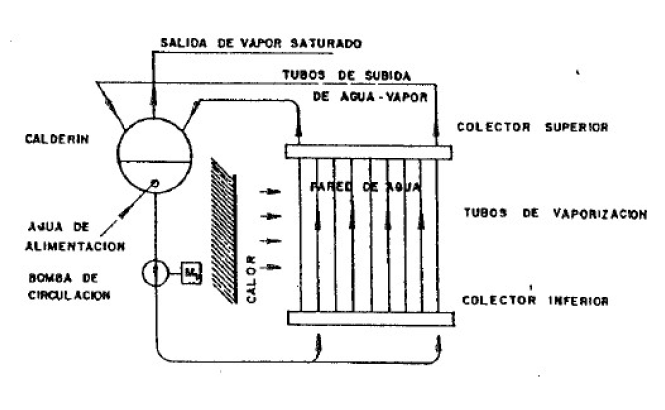
\includegraphics[width=0.7\linewidth]{res/tema10/autotubu}
	\label{fig:autotubu}
\end{figure}



Las calderas de circulación forzada se denominan también generadores de vapor o calderas de circuito abierto. En ellas el agua es impulsada unicamente por una bomba de alta presión (llega a los 230 bar).
\section{Calderín.}
Tiene como objetivo separar las fases líquida y gaseosa por medio de equipos separadores de la mezcla procedente del evaporador para conseguir un vapor seco con grado de humedad $<10\%$. 



El calderín se sitúa en la parte más alta de la caldera y es un gran cilindro horizontal de unos 2 metros de diámetro y 15m de longitud. El cuerpo del calderín se hace de acero especial de manera que soporte las tensiones térmicas (espesor de 10cm):
\begin{itemize}
	\item [-] Interior: 175 bar y 350\grado.
	\item [-] Exterior: 1 bar y 30\grado.
\end{itemize}




El volumen de agua existente en el calderín constituye una gran reserva de
seguridad que amortigua los efectos de los transitorios de carga.



Para realizar el secado del vapor húmedo se centrifuga este mismo de manera que se separa el vapor de la humedad por diferencia de pesos. Tras ello, el vapor seco se pasa el vapor seco a través de chapas apiladas que eliminan el agua residual y llena el pleno gaseoso del calderín. Por otra parte, la humedad pasa a formar parte de la piscina líquida.
\begin{figure}[H]
	\centering
	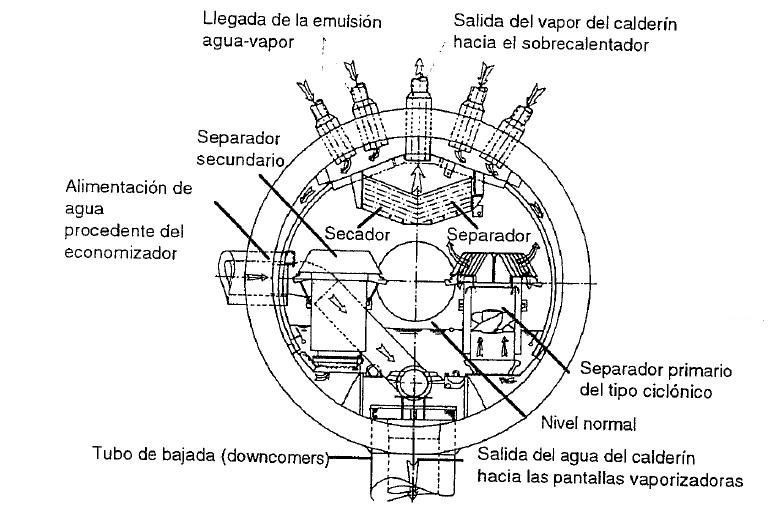
\includegraphics[width=0.7\linewidth]{res/tema10/calderin}
	\label{fig:calderin}
\end{figure}

\section{Sobrecalentadores.}
Son los intercambiadores de haces tubulares que están sometidos a mayores temperaturas,
ya que por su interior circula vapor  y por el
exterior lo hacen los gases de combustión.




Constructivamente, son haces de tubos con diámetros de unos 50mm distribuidos en bancos de profundidad de unos pocos metros y con una ligera separación entre ellos. El vapor circula por su interior a velocidades comprendidas entre 20 y 35 $\frac{m}{s}$.





En función de la temperatura se emplean diferentes materiales. Hasta 540\grado se usan aceros ferríticos de baja aleación (con algo de Cromo, Molibdeno y
Vanadio). Mientras que para temperaturas hasta los 600\grado se sustituyen por aceros austeníticos
(inoxidables, con alto contenido en Cromo 18\% y Níquel 8\%) con un coste notablemente
mayor.




El sobrecalentador se divide en el primario (radiación) y secundario (convección).


\section{Recalentadores.}
En las calderas que alimentan turbinas de dos o tres cuerpos ( alta, media y baja presión)
existen los recalentadores, destinados a recalentar el vapor parcialmente expansionado en el
cuerpo de alta presión.


Los recalentadores tienen características similares a los sobrecalentadores aunque trabajan a aproximadamente una cuarta parte de la presión. Tienen una pérdida de carga de aproximadamente un 4\%.

\section{Economizador.}
Tiene como objetivo reducir el consumo de combustible de la instalación y evitar tensiones térmicas en el calderín. Se sitúa en el extremo final de la zona de recuperación de calor en la caldera.


Es este punto la temperatura de los humos todavía es elevada (por encima de 500\grado) y el
modo predominante de transmisión de calor es por convección.

El economizador es un intercambiador sin mezcla del tipo agua/gas formado por un conjunto de
haces tubulares.

\section{Líneas de vapor.}
Una línea de vapor principal o vapor vivo conduce el vapor sobrecalentado desde la caldera hasta la turbina
de alta presión. La línea de vapor vivo es de gran longitud ya que se extiende desde la parte alta del
edificio de caldera hasta la cota de operaciones en la nave de turbinas.



Una línea de vapor recalentado caliente transporta el vapor ya recalentado hasta la turbina de media presión.



Las tuberías que se emplean para estos circuitos suelen tener diámetros en torno a los 80cm y deben soportar las máximas temperaturas de vapor. Además, se envuelven en aislante térmico para reducir las pérdidas en las tuberías.

\begin{table}[H]
	\centering
	\renewcommand{\arraystretch}{1.5}
	\begin{tabular}{cccc}
		\hline
		Línea&Caudal de vapor ($\frac{t}{h}$)&Presión máxima (bar)&Tª máxima (\grado)\\
		\hline
		Vapor vivo&1900&170&538\\
		\hline
		Vapor recalentado frío&1900&36&421\\
		\hline
		Vapor recalentado caliente&1750&34&538\\
		\hline
	\end{tabular}
\end{table}
\section{Turbinas de vapor.}
La turbina de vapor está destinada a proporcionar potencia mecánica para
mover un generador eléctrico y producir electricidad. Constituye un conjunto denominado
turbogenerador que tiene una velocidad de giro de 1500 o 3000rpm.


El vapor llega a la turbina a alta presión y temperatura (por encima de los 175 bar y 545 \grado) con un alto valor entálpico de 3400$\frac{kJ}{kg}$. De esta forma, durante la expansión, y de forma escalonada según el número de etapas de alabes el vapor transfiere su energía a la turbina generando potencia. 





Si la turbina se compone de más cuerpos la potencia mecánica total es la suma de potencias y si se realizan extracciones l caudal se resta la porción de
vapor extraído.


Debido a la gran longitud que puede alcanzar el turbogrupo ( 20 a 40 m), se divide en tres o
más partes , correspondientes a los cuerpos de la turbina ( alta, media y baja presión) y el alternador. La disposición más común es en eje tamdem-compound , en el que todos los rotores están
alineados en un sólo eje.



Cuantas más etapas tenga una turbina menor será la temperatura de la salida. Sigue la siguiente expresión:
\[\frac{T_ {entrada}}{n_{etapas}}=T_{salida}\]
\subsection{Clasificación de turbinas de vapor.}
Según la dirección del flujo se habla de turbinas axiales o radiales.


Según el tipo de escalonamiento se habla de turbinas tipo Curtis (escalonamiento de velocidad) o de tipo Rateau (escalonamiento de presión). 


\begin{figure}[H]
	\begin{minipage}{0.50\textwidth}
		\centering
		\textbf{Escalonamiento de velocidad.}
		\begin{figure}[H]
			\centering
			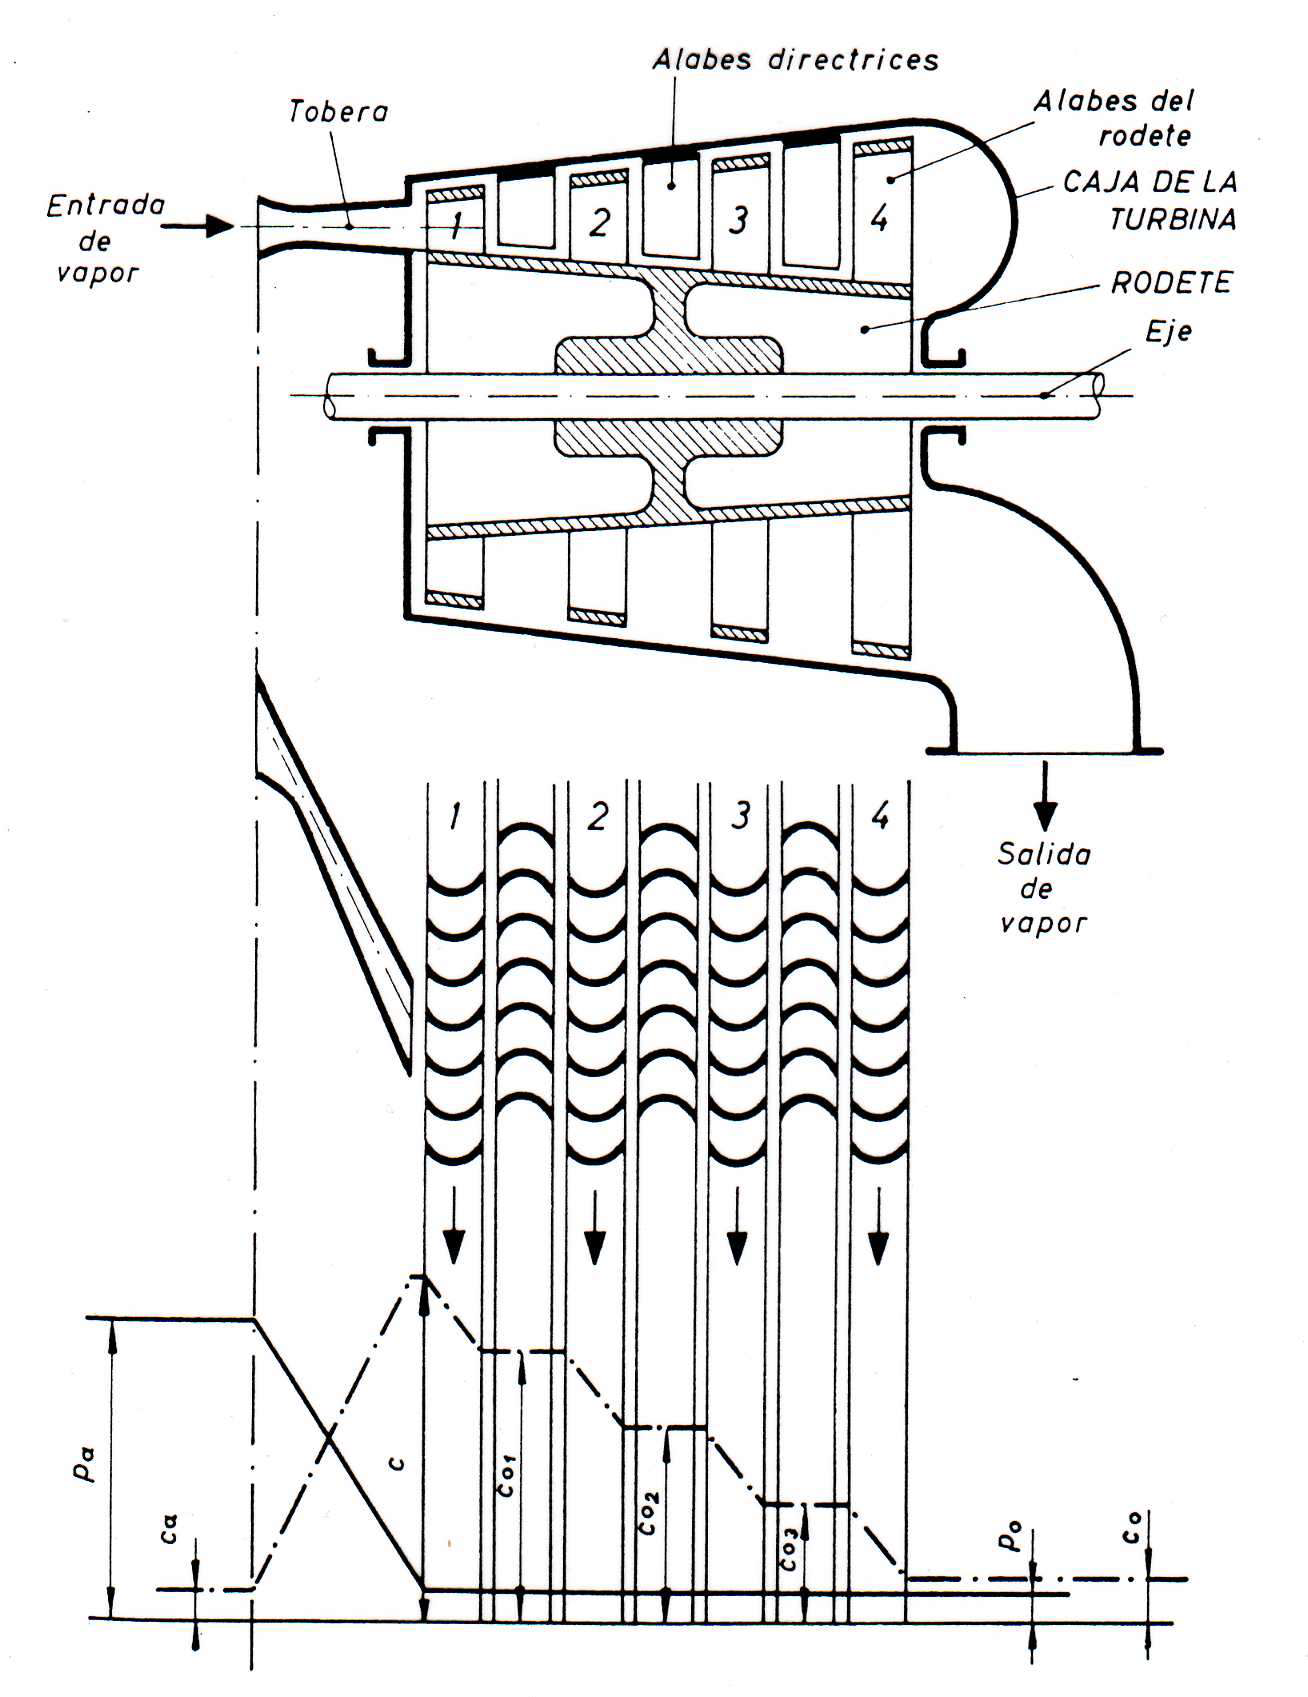
\includegraphics[width=0.7\linewidth]{res/tema10/escVel}
			\label{fig:escvel}
		\end{figure}
	\end{minipage}
	\begin{minipage}{0.50\textwidth}
		\centering
		\textbf{Escalonamiento de presión.}
		\begin{figure}[H]
			\centering
			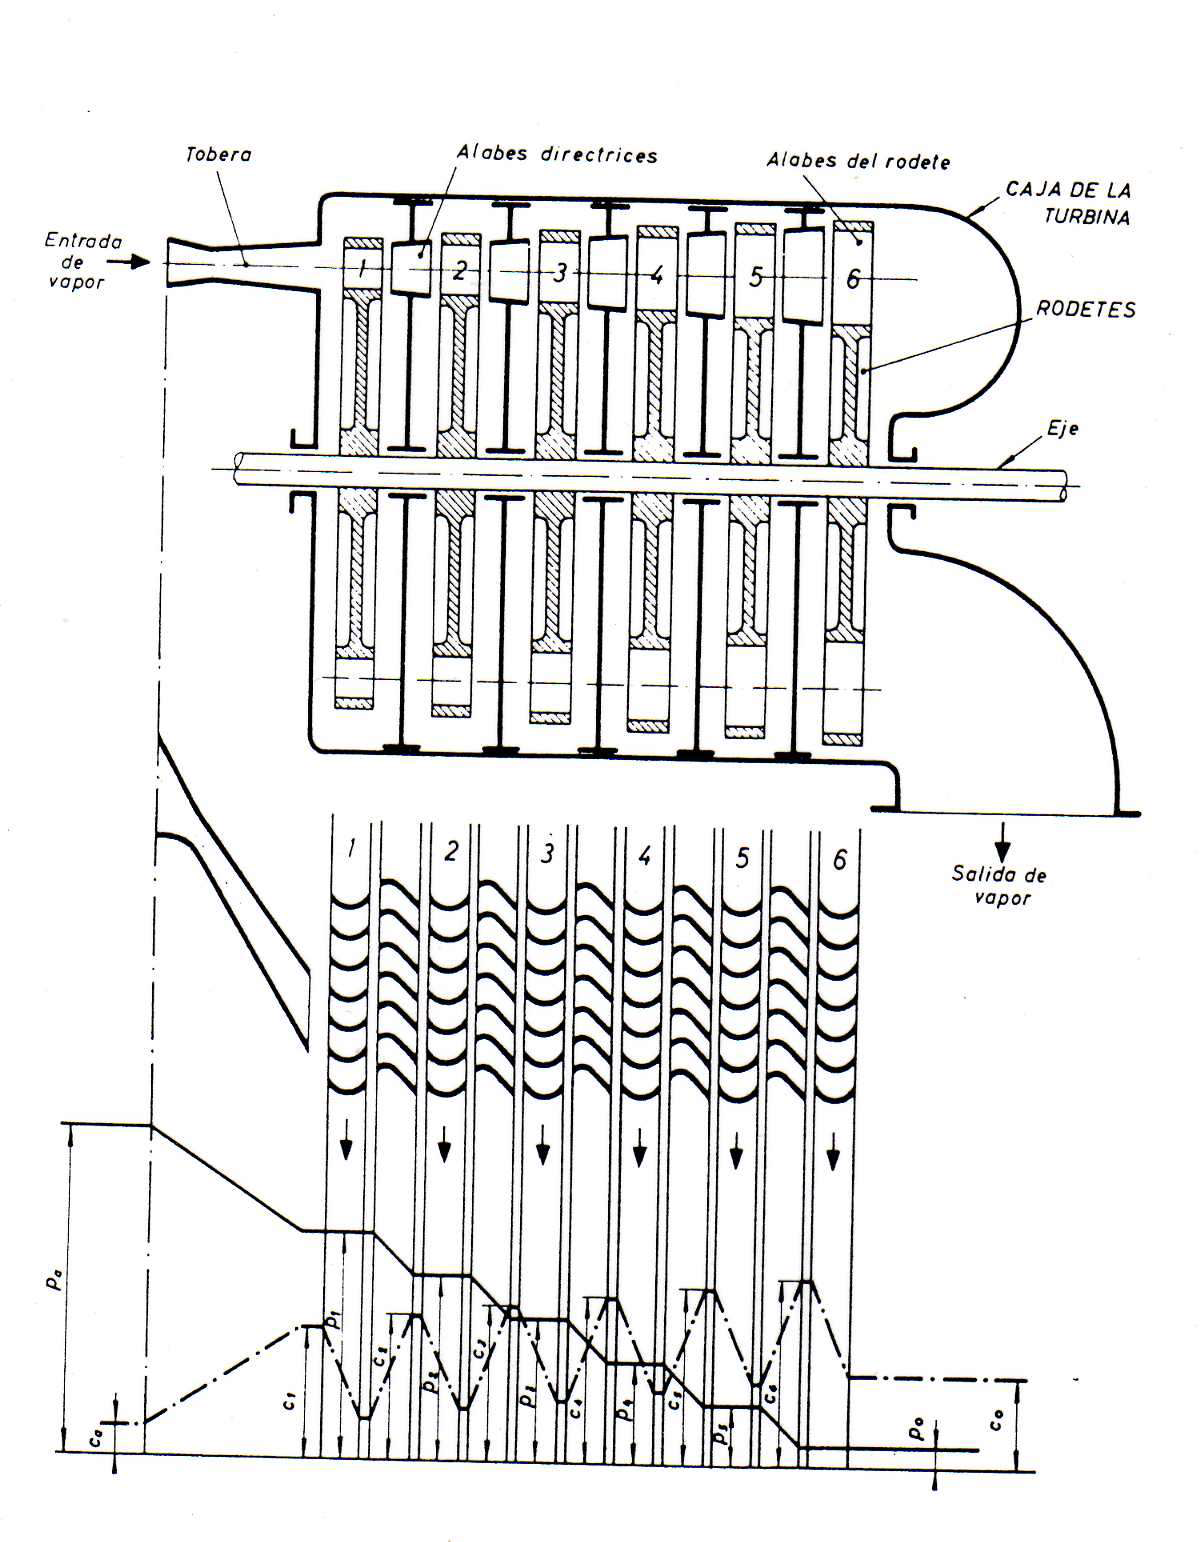
\includegraphics[width=0.7\linewidth]{res/tema10/escpre}
			\label{fig:escpre}
		\end{figure}
	\end{minipage}
\end{figure}








Según el estado del vapor a la entrada de la turbina, puede ser de vapor vivo ( cuerpo de alta presión),
vapor saturado (cuerpo de media presión) o vapor recalentado (cuerpo de baja presión).





\subsection{Recorrido del vapor a través de la turbina.}
El vapor sobrecalentado se conduce a la turbina de alta presión, pasando primero por las válvulas de parada y después por las válvulas de regulación. Tras ello, el vapor pasa por los sucesivos escalonamientos produciendo un trabajo específico
por unidad de masa (salto entálpico). Este vapor sale con una temperatura y presión más baja.


Una vez sale el vapor de la zona de alta presión se recalienta hasta una temperatura similar a la del vapor vivo y, a una presión inferior (50 bar) que será conducida al cuerpo de media presión.

Por último, el vapor expansionado a 10bar se puede introducir en los cuerpos de baja presión simétricos (tubería crossover) o bien ser recalentado.
\section{Condensadores.}
Tiene como función condensar el vapor procedente de la turbina. El calor latente del vapor se transfiere al medio refrigerante para ser disipado a la atmósfera.

Esto supone que, aproximadamente, dos terceras partes del contenido energético del combustible
son evacuadas directamente al condensador.


La temperatura a la que el vapor se condensa depende en gran parte de la temperatura del foco
frío, que no permanece constante en el tiempo. Las variaciones del foco frío pueden ser
estacionales.



Se trata de un equipo esencial, ya que sus condiciones determinan el salto entálpico disponible del
vapor. Para conseguir un máximo de aprovechamiento de la expansión en turbina el condensador trabaja
en condiciones de vacío, a una presión inferior a la atmosférica.


Normalmente, como agente refrigerante, la mayor parte de los condensadores emplean agua.

En función de la disposición de los tubos implicados se habla de intercambiadores de mezcla y de intercambiadores de superficie (más comunes en centrales térmicas).

\begin{itemize}
	\item [-] En los intercambiadores de mezcla existe contacto íntimo entre los fluidos a calentar y condensar.
	\item [-] En los intercambiadores de superficie una barrera física separa ambos fluidos.
\end{itemize}

\subsection{Condensadores de superficie.}
El vapor procedente del
escape de la turbina inunda el vacío de la carcasa , mientras que el agua de refrigeración
fluye por el interior de los tubos con la presión necesaria para vencer las pérdidas de carga.



Como consecuencia del gran volumen específico del vapor a baja presión (20$\frac{m^3}{
	kg}$ a 50
mmHg) y el enorme flujo de vapor a tratar (700 $\frac{t}{h}$ en un grupo de 350 MW ) el tamaño del
condensador es considerable.



El condensador consta de:
\begin{itemize}
	\item [-] Uno o varios cuerpos, generalmente de acero, en los que el vapor es descargado y donde se
	aloja el haz tubular.
	\item [-] Las cajas de agua situadas en los extremos del condensador que sirven para distribuir de
	forma homogénea el caudal del agua de circulación entre todos los tubos.
	\item [-] Haz de tubos , generalmente de aleaciones de cobre, dispuestos verticalmente en forma de
	tresbolillo.
	\item [-] En la zona inferior se ubica una balsa o foso, denominado pozo de condensado o pozo
	caliente, que recoge el vapor ya condensado.
\end{itemize}
\begin{figure}[H]
	\centering
	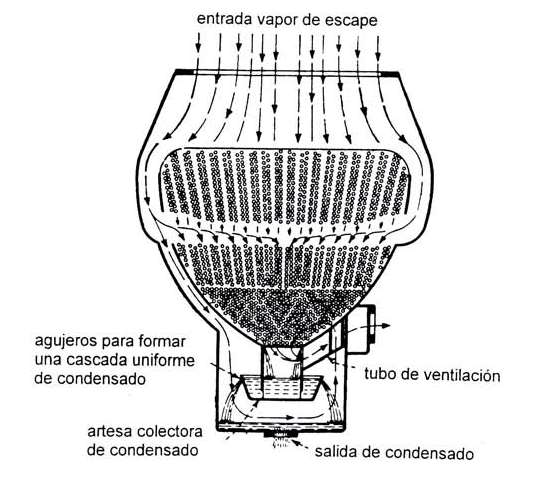
\includegraphics[width=0.7\linewidth]{res/tema10/condensador}
	\label{fig:condensador}
\end{figure}

\section{Sistema de alimentación.}
El vapor condensado se debe bombear nuevamente a la caldera en las condiciones adecuadas de presión y temperatura.



Este bombeo en fase líquida se realiza normalmente en dos etapas, que dan origen a los
sistemas de agua de condensado (desde el pozo caliente del condensador hasta el
desgasificador) y de agua de alimentación (desde el tanque del desgasificador hasta el
economizador de caldera).
\section{Desgasificador.}
Se encarga de que el agua de alimentación  alcance la temperatura de ebullición correspondiente a la presión de vapor de
extracción de la turbina. Para ello, en el desgasificador se debe garantizar un calentamiento uniforme, la desgasificación y la extracción de incondensables (burbujas en al agua).


El calentamiento del agua de condensado con vapor de caldeo se efectúa en diferentes
etapas de acuerdo con el número de extracciones de turbina ya que el rendimiento del ciclo aumenta al emplear el vapor de turbina para calentar el agua del
ciclo.



Las líneas del sistema de extracciones de vapor, que conducen este hasta los calentadores,
van provistas de válvulas de cierre y válvulas de retención controladas para evitar que se
pudiese revertir el flujo de vapor, lo que podría provocar el embalamiento de la turbina si el
grupo se desacopla de la red.


\section{Calentadores de agua de ciclo.}
Habitualmente son de dos pasos por tubo por lo que las cámaras de entrada y salida están
localizadas en el mismo extremo del cambiador. Las velocidades suelen ser de 3$\frac{m}{s}$.
\begin{figure}[H]
	\centering
	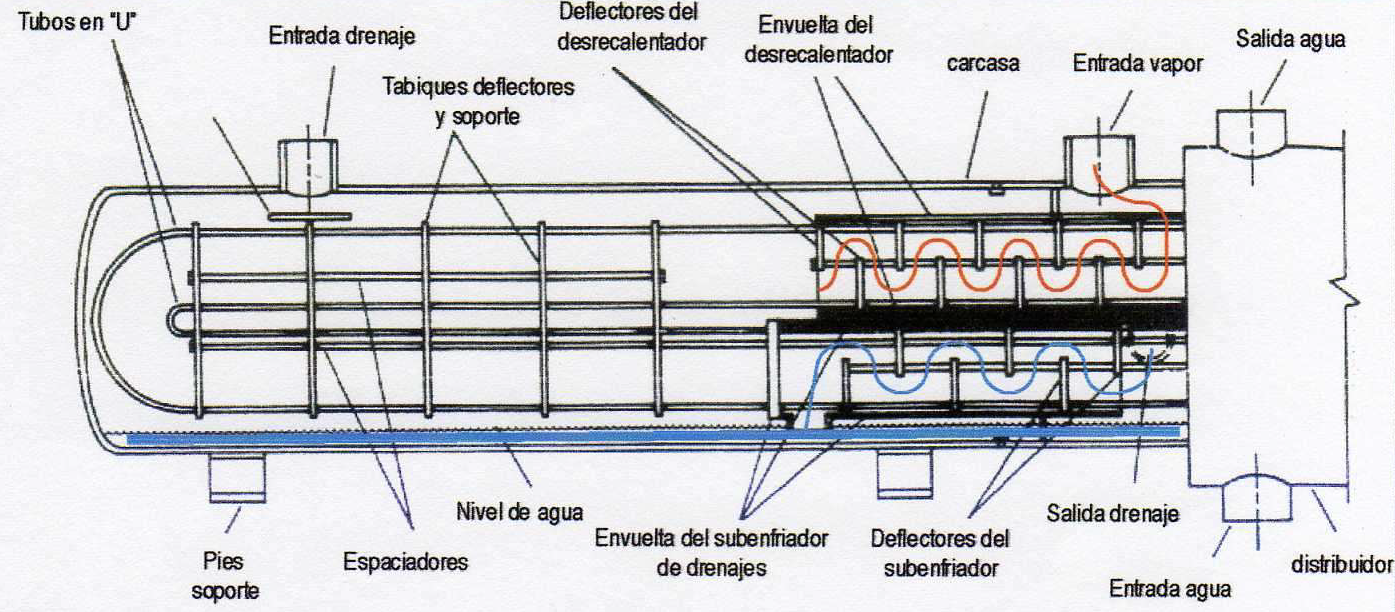
\includegraphics[width=1\linewidth]{res/tema10/calentador}
	\label{fig:calentador}
\end{figure}

Las características geométricas de los cambiadores suelen ser las siguientes:
\begin{table}[H]
	\centering
	\renewcommand{\arraystretch}{1.5}
	\begin{tabular}{cc}
		\hline
		Propiedad&Magnitud\\
		\hline
		Longitud&6-9m\\
		\hline
		Diámetro de la carcasa&0,75-1,5m\\
		\hline
		Número de tubos&400-1200\\
		\hline
		Diámetro tubos&14-146mm\\
		\hline
		Superficie total de calefacción&300-1000$m^2$\\
		\hline
		
	\end{tabular}
\end{table}

\section{Sistema de refrigeración.}
El agua de circulación debe evacuar el calor latente de condensación y, por ello, son necesarios circuitos de refrigeración. Suele provocar que el agia refrigerante tenga una subida de aproximadamente 10\grado.


El sistema de circulación tiene tres disposiciones básicas:
\begin{itemize}
	\item [-] \textbf{Circuito abierto}: el agua se  obtiene aguas arriba de un río y se expulsa aguas abajo.
	\item [-] \textbf{Circuito cerrado}: el agua no sale del circuito y se emplean torres de refrigeración.
	\item [-] \textbf{Circuito mixto}: se obtiene agua aguas abajo de un río y se emplean torres de refrigeración.
\end{itemize}
	
Las bombas de agua están situadas en la toma de agua en un edificio denominado casa de bombas. La toma de aguas debe disponer dispositivos de filtrado adecuados. Las bombas por su parte, suelen ser centrífugas, diseñadas para un gran caudal y tener rendimientos altos.


Por otro lado, las torres de refrigeración son las encargadas del intercambio de materia y energía con el aire ambiente. Por ello, se debe maximizar la cantidad de agua en contacto.


Para ello, el aire asciende por el interior de la torre y el agua desciende por gravedad.


En función de la forma de crear el tiro se distingue entre:
\begin{itemize}
	\item [-] \textbf{Tiro natural}: se basan en la diferencia de densidad entre el aire caliente dentro de la torre y el aire más fresco en el exterior para generar un flujo de aire. Pueden ser hiperbólicas, cilíndricas o troncocónicas.
	\item [-] \textbf{Tiro mecánico}: se basan en el uso de ventiladores para enfriar el agua. Pueden ser de tipo inducido o forzado.
	\item [-] \textbf{Tiro asistido}: es un sistema mixto entre los anteriores.
\end{itemize}

En función del flujo relativo agua-aire:
\begin{itemize}
	\item [-] Flujo en contracorriente.
	\item [-] Flujo cruzado.
\end{itemize}
\section{Tratamiento del agua de alimentación-circuito de refrigeración.}
El agua empleada en una central térmica no debe tener sales e impurezas, pues ello, reduciría considerablemente la vida útil de los distintos componentes del circuito. Por tanto, el agua debe tener las siguientes características:
\begin{table}[H]
	\centering
	\renewcommand{\arraystretch}{1.5}
	\begin{tabular}{ccc}
		\hline
		Elemento/propiedad&Cantidad &Unidades\\
		\hline
		Sólidos disueltos&0,05 &p.p.m\\
		\hline
		Oxígeno disuelto&0,007  &p.p.m\\
		\hline
		Sílice&0,02 &p.p.m\\
		\hline
		Hierro&0,01&p.p.m\\
		\hline
		Cobre& 0,002&p.p.m\\
		\hline
		Dureza&0 &p.p.m\\
		\hline
		$CO_2$&0 &p.p.m\\
		\hline
		Materia orgánica& 0&p.p.m\\
		\hline
		pH&8,5-9,2 & -\\
		\hline
		Conductividad& 20,1&$\frac{\mu s}{cm}$\\
		\hline
	\end{tabular}
\end{table}

Para conseguir estas propiedades se realiza el siguiente proceso de tratamiento:
\begin{enumerate}
	\item Pretratamiento del agua.
	\item Desmineralización del agua pretratada.
	\item Tratamiento del condensado.
	\item Tratamientos adicionales.
	\begin{enumerate}
		\item Clarificación, coagulación y sedimentación.
		\item Ablandamiento.
		\item Esterilización.
		\item Filtración.
	\end{enumerate}
\end{enumerate}




Si no se trata el agua pueden ocurrir las siguientes acciones perjudiciales:
\begin{itemize}
	\item [-] \textbf{Incrustaciones}: son debidas principalmente a los cationes iónicos disueltos. Lo cual produce:
	\begin{itemize}
		\item Disminución del coeficiente de transmisión del calor.
		\item Reducción de la sección útil de las tuberías.
		\item Rotura de tubos por sobrecalentamiento.
	\end{itemize}
	\item [-] \textbf{Corrosiones}: se deben principalmente al oxígeno y en menor medida al dióxido de carbono y otros ácidos minerales. Lo cual produce:
	\begin{itemize}
		\item Disolución del metal de la caldera, economizador, condensador y tuberías.
		\item Los gases insolubles se eliminan en el desgasificador.
		\item El oxígeno residual puede reaccionar con sulfito sódico para dar sulfatos o hidracina para dar agua y nitrógeno libre.
		\item Para contrarrestar la acidificación producida por el dióxido de carbono se inyecta amoniaco. 
	\end{itemize}
\end{itemize}
\section{Control de una central térmica.}
El control de una central térmica se puede realizar siguiendo tres criterios:
\begin{itemize}
	\item [-] \textbf{Turbina siguiendo a caldera}: se utiliza cuando el combustible que se desea gastar no se puede almacenar y se debe consumir a medida que se produce. Centrales que aprovechan el gas de alto horno.
	\item [-] \textbf{Caldera siguiendo a turbina}: es el más extendido y tiene como objetivo satisfacer la demanda eléctrica. 
	\item [-] \textbf{Control coordinado}:
	la señal de demanda de energía actúa simultáneamente sobre caldera y turbina.
\end{itemize}


Los principales controles de una central térmica son:
\begin{itemize}
	\item [-] Control de combustión.
	\item [-] Control de temperatura de vapor sobrecalentado y recalentado.
	\item [-] Control de agua de alimentación.
	\item [-] Control de condensado y drenaje de calentadores.
	\item [-] Control de bypass de alta y baja presión de la turbina.
\end{itemize}

El control de combustión consiste en regular la cantidad de aire y combustible que entran en el hogar, en función de la consigna de potencia eléctrica a suministrar.